


\documentclass[aspectratio=169,xcolor=dvipsnames]{beamer}
%\usetheme{SimplePlus}

\usepackage{hyperref}
\usepackage{graphicx} % Allows including images
\usepackage{booktabs} % Allows the use of \toprule, \midrule and \bottomrule in tables

%----------------------------------------------------------------------------------------
%	TITLE PAGE
%----------------------------------------------------------------------------------------
\title[Flowmåling] {Strømningsmåling}

%\subtitle{Subtitle}

\author[Fred-Olav] {Fred-Olav Mosdal}

\institute[Gand VGS] % Your institution as it will appear on the bottom of every slide, may be shorthand to save space
{
    Gand VGS \\
    VG3 Automasjon
}
\date{\today} % Date, can be changed to a custom date
\begin{document}
\maketitle
\begin{frame}
	\frametitle{Hastighetsbaserte strømningsmålere}

	$$\includegraphics[height=4cm]{fluids_01.eps}$$
$$A_1 \overline{v_1} = A_2 \overline{v_2}$$
\end{frame}

%
%If the density of the fluid is not subject to change as it travels through the pipe (a very good assumption for liquids), we may simplify the Law of Continuity by eliminating the density terms from the equation:
%
%
%The product of cross-sectional pipe area and average fluid velocity is the volumetric flow rate of the fluid through the pipe ($Q = A\overline{v}$).  This tells us that fluid velocity will be directly proportional to volumetric flow rate given a known cross-sectional area and a constant density for the fluid flowstream.  Any device able to directly measure fluid velocity is therefore capable of inferring volumetric flow rate of fluid in a pipe.  This is the basis for \textit{velocity-based} flowmeter designs.
%
%
%
%
%
%
%
%\filbreak
%\subsection{Turbine flowmeters}
\begin{frame}
	\frametitle{Turbin strømningsmålere}

	$$\includegraphics[height=7cm]{flow51.eps}$$
\end{frame}

%
%\textit{Turbine} flowmeters use a free-spinning turbine wheel to measure fluid velocity, much like a miniature windmill installed in the flow stream.  The fundamental design goal of a turbine flowmeter is to make the turbine element as free-spinning as possible, so no torque will be required to sustain the turbine's rotation.  If this goal is achieved, the turbine blades will achieve a rotating (tip) velocity directly proportional to the linear velocity of the fluid, whether that fluid is a gas or a liquid: \index{Turbine flow element}
%
%$$\includegraphics{flow51.eps}$$
%
%\filbreak
%
%The mathematical relationship between fluid velocity and turbine tip velocity -- assuming frictionless conditions -- is a ratio defined by the \textit{tangent} of the turbine blade angle:
%
%$$\includegraphics{flow76.eps}$$

%
%For a 45$^{o}$ blade angle, the relationship is 1:1, with tip velocity equaling fluid velocity.  Smaller blade angles (each blade closer to parallel with the fluid velocity vector) result in the tip velocity being a fractional proportion of fluid velocity.
%
%\filbreak
%
%Turbine tip velocity is quite easy to sense using a magnetic sensor, generating a voltage pulse each time one of the ferromagnetic turbine blades passes by.  Traditionally, this sensor is nothing more than a coil of wire in proximity to a stationary magnet, called a \textit{pickup coil} or \textit{pickoff coil} because it ``picks'' (senses) the passing of the turbine blades.  Magnetic flux through the coil's center increases and decreases as the passing of the steel turbine blades presents a varying reluctance (``resistance'' to magnetic flux), causing voltage pulses equal in frequency to the number of blades passing by each second.  It is the \textit{frequency} of this signal that represents fluid velocity, and therefore volumetric flow rate. \index{Pickup coil}  \index{Pickoff coil}
%
%A cut-away demonstration model of a turbine flowmeter is shown in the following photograph.  The blade sensor may be seen protruding from the top of the flowtube, just above the turbine wheel:
%
%$$\includegraphics[width=5in]{turbineflowmeter1.eps}$$
\begin{frame}
	\frametitle{Turbin strømningsmålere}

	$$\includegraphics[height=7cm]{turbineflowmeter1.eps}$$
\end{frame}
%
%Note the sets of ``flow conditioner'' vanes immediately before and after the turbine wheel in the photograph.  As one might expect, turbine flowmeters are very sensitive to \textit{swirl} in the process fluid flowstream.  In order to achieve high accuracy, the flow profile must not be swirling in the vicinity of the turbine, lest the turbine wheel spin faster or slower than it should to represent the velocity of a straight-flowing fluid.  A minimum straight-pipe length of 20 pipe diameters upstream and 5 pipe diameters downstream is typical for turbine flowmeters in order to dissipate swirl from piping disturbances.
%
%Mechanical gears and rotating cables have also been historically used to link a turbine flowmeter's turbine wheel to indicators.  These designs suffer from greater friction than electronic (``pickup coil'') designs, potentially resulting in more measurement error (less flow indicated than there actually is, because the turbine wheel is slowed by friction).  One advantage of mechanical turbine flowmeters, though, is the ability to maintain a running total of gas usage by turning a simple odometer-style totalizer.  This design is often used when the purpose of the flowmeter is to track total fuel gas consumption (e.g. natural gas used by a commercial or industrial facility) for billing.
%
%\filbreak
%
%In an electronic turbine flowmeter, volumetric flow is directly and linearly proportional to pickup coil output frequency.  We may express this relationship in the form of an equation:
%
\begin{frame}
	\frametitle{Turbin strømningsmålere}
$$f = kQ$$

Der,
\\
$f$ = Frequency of output signal (Hz, equivalent to pulses per second)
\\
$Q$ = Volumetric flow rate (e.g. liter per second)
\\
$k$ = ``K'' factor of the turbine element (e.g. pulses per liter)
\\
$$\left[\hbox{Pulses} \over \hbox{s} \right] = \left[\hbox{Pulses} \over \hbox{liter} \right] \left[\hbox{liter} \over \hbox{s} \right]$$
\\
$$Q = {f \over k}$$

\end{frame}
\begin{frame}
	\frametitle{Elektromagnetisk strømningsmåler}

	$$\includegraphics[height=7cm]{flow57.eps}$$
\end{frame}

%
%The direction of liquid flow cuts perpendicularly through the lines of magnetic flux, generating a voltage along an axis perpendicular to both.  Metal electrodes opposite each other in the pipe wall intercept this voltage, making it readable to an electronic circuit.
%
%\filbreak
%
%A voltage induced by the linear motion of a conductor through a magnetic field is called \textit{motional EMF}, the magnitude of which is predicted by the following formula (assuming perfect perpendicularity between the direction of velocity, the orientation of the magnetic flux lines, and the axis of voltage measurement):  \index{Motional EMF}
%
\begin{frame}
	\frametitle{Elektromagnetisk strømningsmåler}
$$\mathcal{E} = Blv$$

Der,
\\
$\mathcal{E}$ = Motional EMF (volts)
\\
$B$ = Magnetic flux density (Tesla)
\\
$l$ = Length of conductor passing through the magnetic field (meters)
\\
$v$ = Velocity of conductor (meters per second)
\\
\vskip 10pt

\end{frame}

%
%Assuming a fixed magnetic field strength (constant $B$) and an electrode spacing equal to the fixed diameter of the pipe (constant $l = d$), the only variable capable of influencing the magnitude of induced voltage is velocity ($v$).  In our example, $v$ is not the velocity of a wire segment, but rather the average velocity of the liquid flowstream ($\overline{v}$).  Since we see that this voltage will be proportional to average fluid velocity, it must also be proportional to volumetric flow rate, since volumetric flow rate is also proportional to average fluid velocity\footnote{This is an application of the transitive property in mathematics: if two quantities are both equal to a common third quantity, they must also be equal to each other.  This property applies to proportionalities as well as equalities: if two quantities are proportional to a common third quantity, they must also be proportional to each other.}.  Thus, what we have here is a type of flowmeter based on electromagnetic induction.  These flowmeters are commonly known as \textit{magnetic flowmeters} or simply \textit{magflow meters}. \index{Magnetic flowmeter}
%
%We may state the relationship between volumetric flow rate ($Q$) and motional EMF ($\mathcal{E}$) more precisely by algebraic substitution.  First, we will write the formula relating volumetric flow to average velocity, and then manipulate it to solve for average velocity:
%
\begin{frame}
	\frametitle{Elektromagnetisk strømningsmåler}
$$Q = A\overline{v}$$
\\
$${Q \over A} = \overline{v}$$
\\
$$\mathcal{E} = Bd\overline{v}$$
\\
$$\mathcal{E} = Bd {Q \over A}$$
\\
$$\mathcal{E} = {BdQ \over A}$$

\end{frame}

%
%Next, we re-state the motional EMF equation, and then substitute $Q \over A$ for $\overline{v}$ to arrive at an equation relating motional EMF to volumetric flow rate ($Q$), magnetic flux density ($B$), pipe diameter ($d$), and pipe area ($A$):
%
%
%\filbreak
%
%Since we know this is a circular pipe, we know that area and diameter are directly related to each other by the formula $A = {\pi d^2 \over 4}$.  Thus, we may substitute this definition for area into the last equation, to arrive at a formula with one less variable (only $d$, instead of both $d$ and $A$):
%
\begin{frame}
	\frametitle{Elektromagnetisk strømningsmåler}
$$\mathcal{E} = {BdQ \over {\pi d^2 \over 4}}$$
\\
$$\mathcal{E} = {BdQ \over 1} {4 \over {\pi d^2}}$$
\\
$$\mathcal{E} = {4BQ \over {\pi d}}$$
\\
$$Q = {\pi d \mathcal{E} \over 4B}$$
\\
$$Q = k {\pi d \mathcal{E} \over 4B}$$

\end{frame}
%
%If we wish to have a formula defining flow rate $Q$ in terms of motional EMF ($\mathcal{E}$), we may simply manipulate the last equation to solve for $Q$:
%
%
%This formula will successfully predict flow rate only for absolutely perfect circumstances.  In order to compensate for inevitable imperfections, a ``proportionality constant'' ($k$) is usually included in the formula\footnote{The colloquial term in the United States for this sort of thing is \textit{fudge factor}.}:
%
%
%\noindent
%Der,
%
%$Q$ = Volumetric flow rate (cubic meters per second)
%
%$\mathcal{E}$ = Motional EMF (volts)
%
%$B$ = Magnetic flux density (Tesla)
%
%$d$ = Diameter of flowtube (meters)
%
%$k$ = Constant of proportionality
%
%\vskip 10pt
%
%Note the linearity of this equation.  Nowhere do we encounter a power, root, or other non-linear mathematical function in the equation for a magnetic flowmeter.  This means no special characterization is required to calculate volumetric flow rate.
%
%A few conditions must be met for this formula to successfully infer volumetric flow rate from induced voltage:
%
%\begin{itemize}
%\item The liquid must be a reasonably good conductor of electricity (\textit{note: it is okay if the conducting fluid contains some non-conducting solids; the conductive fluid surrounding the non-conducting solid matter still provides electrical continuity between the electrodes necessary for induction})
%\item The pipe must be completely filled with liquid to ensure contact with both probes as well as to ensure flow across the entire cross-section of the pipe
%\item The flowtube must be properly grounded to avoid errors caused by stray electric currents in the liquid
%\end{itemize}
%
%\filbreak
%
%The first condition is met by careful consideration of the process liquid prior to installation.  Magnetic flowmeter manufacturers will specify the minimum conductivity value of the liquid to be measured.  The second and third conditions are met by correct installation of the magnetic flowtube in the pipe.  The installation must be done in such a way as to guarantee full flooding of the flowtube (no gas pockets).  The flowtube is usually installed with electrodes across from each other horizontally (never vertically!) so even a momentary gas bubble will not break electrical contact between an electrode tip and the liquid flowstream.  The following photograph shows how \textit{not} to install magnetic flowmeters:
%
%$$\includegraphics[width=5in]{magflow7.eps}$$
\begin{frame}
	\frametitle{Elektromagnetisk strømningsmåler montering}

	$$\includegraphics[height=7cm]{magflow7.eps}$$
\end{frame}

%
%Note in this example how the electrodes are vertically oriented instead of horizontal, because the pipes for these two magnetic flowmeters were placed too close\footnote{The obvious solution to this problem -- relocating the pipes to give more clearance between flowmeters -- would be quite expensive given the large pipe sizes involved.  A ``compromise'' solution is to tilt the magnetic flowtubes as far as possible without the electrodes touching the adjacent flowtube.  Horizontal electrode installation is ideal for horizontal pipes, but an angled installation will be better than a vertical installation.} to allow proper clearance for the protruding electrodes to lie horizontally.  Sadly, poor flowmeter installation is all too common in new projects, as many piping designers and pipefitters are ignorant of flowmeter operating principles.  This is one way instrument engineers and technicians may deter operational problems: by involving themselves in the design phase of a piping system, and helping to educate piping designers.
%
%\vskip 10pt
%
%Magnetic flowmeters exhibit several advantages over other types of flowmeter.  They are fairly tolerant of swirl and other large-scale turbulent fluid behavior, because the induced voltage is proportional only to the \textit{perpendicular} velocity of the conductor, in this case the velocity of the fluid along the centerline of the flowtube.  As such, magnetic flowmeters do not require the long straight-runs of pipe upstream and downstream that orifice plates do, which is a great advantage in many piping systems.  Upstream straight-pipe requirements of 5 diameters and downstream straight-pipe requirements of 3 diameters is typical\footnote{As always, check the manufacturer's literature for specific requirements, as variations do exist for different models and sizes of magtube.}.
%
%Additionally, the wide-open bore of a magnetic flowmeter's tube means there is absolutely nothing to restrict the flow, resulting in extremely low permanent pressure loss.  The lack of any obstruction within the path of fluid flow means magnetic flowmeters are quite tolerant of solids\footnote{Even electrically \textit{non-conducting} solid matter is tolerated well by magnetic flowmeters, since the conducting liquid surrounding the solids still provides continuity from one electrode to the other.} within the liquid flowstream, making them well-suited for measuring such process liquids as wastewater, slurries, wood pulp, and food products which might clog other types of flowmeters.  In fact, magnetic flowmeters are the dominant flowmeter technology used in wastewater, wood pulping, and food processing industries for this very reason.
%
%\vskip 10pt
%
%\filbreak
%
%Electrical conductivity of the process liquid must meet a certain minimum value, but that is all.  It is surprising to some technicians that changes in liquid conductivity have little to no effect on flow measurement accuracy.  It is not as though a doubling of liquid conductivity will result in a doubling of induced voltage!  Motional EMF is strictly a function of physical dimensions, magnetic field strength, and fluid velocity.  
%
%Liquids with poor conductivity present a greater electrical resistance in the voltage-measuring circuit than liquids with good conductivity, but this is of little consequence because the input impedance of the detection circuitry is phenomenally high.  The effect of liquid conductivity on flowmeter operation may be modeled by the following DC circuits:
%
%$$\includegraphics{magflow8.eps}$$
\begin{frame}
	\frametitle{Elektromagnetisk strømningsmåler}

	$$\includegraphics[height=7cm]{magflow8.eps}$$
\end{frame}

%
%Here, a ten-fold (one order of magnitude) change in liquid resistance barely affects the measured voltage (49.995 mV versus 49.95 mV) because the flow transmitter's voltage-sensing electronic circuit has such a high input impedance.  The liquid's equivalent resistance value must increase dramatically beyond the values shown in this example before it will have any significant effect on flow measurement accuracy.
%
%In fact, the only time fluid conductivity is a problem with magnetic flowmeters is when the fluid in question has negligible conductivity.  Such fluids include deionized water (e.g. steam boiler feedwater, ultrapure water for pharmaceutical and semiconductor manufacturing) and oils.  Most aqueous (water-based) fluids work fine with magnetic flowmeters.
%
%\filbreak
%
%Proper grounding of the flowtube is very important for magnetic flowmeters.  The motional EMF generated by most liquid flowstreams is very weak (1 millivolt or less!), and therefore may be easily overshadowed by noise voltage present as a result of stray electric currents in the piping and/or liquid.  To combat this problem, magnetic flowmeters are usually equipped with grounding conductors placed to shunt (bypass) stray electric currents around the flowtube so the only voltage intercepted by the electrodes will be the motional EMF produced by liquid flow, and not voltage drops created by stray currents through the resistance of the liquid.  The following photograph shows a Rosemount model 8700 magnetic flowtube, with two braided\footnote{Braided conductors do a better job of shunting radio-frequency currents, because at very high frequencies the \textit{skin effect} makes the surface area of a conductor a greater factor in its conductivity than its cross-sectional area.}-wire grounding straps clearly visible:
%
%$$\includegraphics[width=4in]{magflow3.eps}$$
\begin{frame}
	\frametitle{Elektromagnetisk strømningsmåler}

	$$\includegraphics[height=7cm]{magflow3.eps}$$
\end{frame}

%
%Note how both grounding straps attach to a common junction point on the flowtube housing.  This common junction point should also be bonded to a functional earth ground when the flowtube is installed in the process line.  On this particular flowtube you can see a stainless steel \textit{grounding ring} on the face of the near flange, connected to one of the braided grounding straps.  An identical grounding ring lays on the other flange, but it is not clearly visible in this photograph.  These rings provide points of electrical contact with the liquid in installations where the pipe is made of plastic, or where the pipe is metal but lined with a plastic material for corrosion resistance.  \index{Grounding, magnetic flowmeters}
%
%\filbreak
%
%If the pipe connecting to a magnetic flowmeter's flowtube is conductive (e.g. metal), grounding may be accomplished by joining the metal pipes' flanges together with grounding straps to a common grounding point on the flowtube body as such:
%
%$$\includegraphics{magflow9.eps}$$
\begin{frame}
	\frametitle{Jording av Elektromagnetisk strømningsmåler}

	$$\includegraphics[height=7cm]{magflow3.eps}$$
\end{frame}
%
%If the pipe connecting to a magnetic flowmeter's flowtube is non-conductive (e.g. plastic) or conductive with an insulating lining (e.g. metal pipe with plastic lining), grounding to the pipe flanges will be pointless.  In order for flowtube grounding to be effective, the grounding conductors must have electrical continuity to the fluid itself.  Special \textit{grounding rings} may be sandwiched between the flanges of non-conducting pipes to provide points of electrical contact with the fluid.  These grounding rings are then joined together with grounding straps to a common grounding point on the flowtube body as such:
%
%$$\includegraphics{magflow10.eps}$$
\begin{frame}
	\frametitle{Jording av Elektromagnetisk strømningsmåler}

	$$\includegraphics[height=7cm]{magflow10.eps}$$
\end{frame}
%
%\vskip 10pt
%
%\filbreak
%
%Some magnetic flowmeters have their signal conditioning electronics located integral to the flowtube assembly.  A couple of examples are shown here (a pair of small Endress+Hauser flowmeters on the left and a large Toshiba flowmeter on the right):  \index{Endress+Hauser magnetic flowmeter}  \index{Toshiba magnetic flowmeter}
%
\begin{frame}
	\frametitle{Elektromagnetisk strømningsmåler}

$$\includegraphics[width=2.5in]{magflow1.eps} \hskip 30pt \includegraphics[width=2.5in]{magflow2.eps}$$
\end{frame}
%
%\filbreak
%
%Other magnetic flowmeters have separate electronics and flowtube assemblies, connected together by shielded cable.  In these installations, the electronics assembly is referred to as the flow transmitter (FT) and the flowtube as the flow element (FE):  \index{Rosemount model 8700 magnetic flowmeter}
%
%$$\includegraphics[width=5in]{magflow4.eps}$$
\begin{frame}
	\frametitle{Elektromagnetisk strømningsmåler}

	$$\includegraphics[height=7cm]{magflow4.eps}$$
\end{frame}
%
%\filbreak
%
%This next photograph shows an enormous (36 inch diameter!) magnetic flow element (black) and flow transmitter (blue, behind the person's hand shown for scale) used to measure wastewater flow at a municipal sewage treatment plant:
%
%$$\includegraphics[height=5in]{magflow6.eps}$$
\begin{frame}
	\frametitle{Elektromagnetisk strømningsmåler}

	$$\includegraphics[height=7cm]{magflow6.eps}$$
\end{frame}
%
%Note the vertical pipe orientation, ensuring constant contact between the electrodes and the water during flowing conditions.
%
%\vskip 10pt
%
%\filbreak
%
%While in theory a permanent magnet should be able to provide the necessary magnetic flux for a magnetic flowmeter to function, this is never done in industrial practice.  The reason for this has to do with a phenomenon called \textit{polarization} which occurs when a DC voltage is impressed across a liquid containing ions (electrically charged molecules).  Electrically-charged molecules (ions) tend to collect near poles of opposite charge, which in this case would be the flowmeter electrodes.  This ``polarization'' would soon interfere with detection of the motional EMF if a magnetic flowmeter were to use a constant magnetic flux such as that produced by a permanent magnet.  A simple solution to this problem is to alternate the polarity of the magnetic field, so the motional EMF polarity also alternates and never gives the fluid ions enough time to polarize.
%
%This is why magnetic flowmeter tubes always employ electromagnet \textit{coils} to generate the magnetic flux instead of permanent magnets.  The electronics package of the flowmeter energizes these coils with currents of alternating polarity, so as to alternate the polarity of the induced voltage across the moving fluid.  Permanent magnets, with their unchanging magnetic polarities, would only be able to create an induced voltage with constant polarity, leading to ionic polarization and subsequent flow measurement errors.
%
%%\filbreak
%
%A photograph of a Foxboro magnetic flowtube with one of the protective covers removed shows these wire coils clearly (in blue): \index{Foxboro magnetic flowtube}
%
%$$\includegraphics[width=4in]{magflow5.eps}$$
\begin{frame}
	\frametitle{Elektromagnetisk strømningsmåler}

	$$\includegraphics[height=7cm]{magflow5.eps}$$
\end{frame}

\begin{frame}
	\frametitle{Vortex strømningsmålere}

	$$\includegraphics[height=6cm]{flow54.eps}$$
\end{frame}

%
%This alternating series of vortices was studied by Vincenc Strouhal in the late nineteenth century and later by Theodore von K\'arm\'an in the early twentieth century.  It was determined that the distance between successive vortices downstream of the stationary object is relatively constant, and directly proportional to the width of the object, for a wide range of Reynolds number values\footnote{It is important to note that the vortex-shedding phenomenon ceases altogether if the Reynolds number is too low.  Laminar flow produces no vortices, but rather stream-line flow around any object placed in its way.}.  If we view these vortices as crests of a continuous wave, the distance between vortices may be represented by the symbol customarily reserved for wavelength: the Greek letter ``lambda'' ($\lambda$). \index{Strouhal, Vincenc}  \index{von K\'arm\'an, Theodore}
%
%$$\includegraphics{flow52.eps}$$
\begin{frame}
	\frametitle{Vortex strømningsmålere}

	$$\includegraphics[height=4cm]{flow52.eps}$$
\end{frame}
%
%The proportionality between object width ($d$) and vortex street wavelength ($\lambda$) is called the \textit{Strouhal number} ($S$), approximately equal to 0.17: \index{Strouhal number}
%
%$$\lambda S = d \hbox{\hskip 50pt} \lambda \approx {d \over 0.17}$$
%
%\filbreak
%
%If a differential pressure sensor is installed immediately downstream of the stationary object in such an orientation that it detects the passing vortices as pressure variations, an alternating signal will be detected:
%
%$$\includegraphics{flow53.eps}$$
\begin{frame}
	\frametitle{Vortex strømningsmålere}

	$$\includegraphics[height=7cm]{flow53.eps}$$
\end{frame}
%
%The \textit{frequency} of this alternating pressure signal is directly proportional to fluid velocity past the object, since the wavelength is constant.  This follows the classic frequency-velocity-wavelength formula common to all traveling waves ($\lambda f = v$).  Since we know the wavelength will be equal to the bluff body's width divided by the Strouhal number (approximately 0.17), we may substitute this into the frequency-velocity-wavelength formula to solve for fluid velocity ($v$) in terms of signal frequency ($f$) and bluff body width ($d$).
%
%$$v = \lambda f$$
%
%$$v = {d \over 0.17} f$$
%
%$$v = {d f \over 0.17}$$
%
%Thus, a stationary object and pressure sensor installed in the middle of a pipe section constitute a form of flowmeter called a \textit{vortex flowmeter}.  Like a turbine flowmeter with an electronic ``pickup'' sensor to detect the passage of rotating turbine blades, the output frequency of a vortex flowmeter is linearly proportional to volumetric flow rate. \index{Vortex flowmeter}
%
%The pressure sensors used in vortex flowmeters are not standard differential pressure transmitters, since the vortex frequency is too high to be successfully detected by such bulky instruments.  Instead, the sensors are typically piezoelectric crystals.  These pressure sensors need not be calibrated, since the amplitude of the pressure waves detected is irrelevant.  Only the frequency of the waves matter for measuring flow rate, and so nearly any pressure sensor with a fast enough response time will suffice.
%
%Like turbine meters, the relationship between sensor frequency ($f$) and volumetric flow rate ($Q$) may be expressed as a proportionality, with the letter $k$ used to represent the constant of proportionality for any particular flowmeter:
%
\begin{frame}
	\frametitle{Vortex strømningsmålere}
$$f = kQ$$
Der,
\\
$f$ = Frequency of output signal (Hz)
\\
$Q$ = Volumetric flow rate (e.g. liter per second)%\footnote{Note that if flow rate is to be expressed in units of gallons per \textit{minute} as is customary, the equation must contain a factor for minutes-to-seconds conversion: $f = {kQ \over 60}$}
\\
$k$ = ``K'' factor of the vortex shedding flowtube (e.g. pulses per liter)

\end{frame}
\begin{frame}
	\frametitle{Vortex strømningsmålere}

	$$\includegraphics[height=7cm]{vortex_flow_03.eps}$$
\end{frame}

%
%The next two photographs show close-up views of the flowtube assembly, front (left) and rear (right): 
%
\begin{frame}
	\frametitle{Vortex strømningsmålere}

$$\includegraphics[width=2.5in]{vortex_flow_01.eps} \hskip 30pt \includegraphics[width=2.5in]{vortex_flow_02.eps}$$
\end{frame}
\begin{frame}
	\frametitle{Koriolis strømningsmåler}

	$$\includegraphics[height=7cm]{coriolis6.eps}$$
\end{frame}

%
%If fluid inside the tube is stagnant (no flow), the tube will simply vibrate back and forth with the applied force.  However, if fluid \textit{flows} through the tube, the moving fluid molecules will experience acceleration as they travel from the anchored base to the tube's rounded end, then experience \textit{deceleration} as they travel back to the anchored base.  This continual acceleration and subsequent deceleration of new mass generates a Coriolis force altering the tube's motion.
%
%\filbreak
%
%This Coriolis force causes the U-tube assembly to \textit{twist}.  The tube portion carrying fluid from the anchored base to the end tends to \textit{lag} in motion because the fluid molecules in that section of the tube are being accelerated to a greater lateral velocity.  The tube portion carrying fluid from the end back to the anchored base tends to \textit{lead} in motion because those molecules are being decelerated back to zero lateral velocity.  As mass flow rate through the tube increases, so does the degree of twisting.  By monitoring the severity of this twisting motion, we may infer the mass flow rate of the fluid passing through the tube:
%
%$$\includegraphics{coriolis9.eps}$$
\begin{frame}
	\frametitle{Koriolis strømningsmåler}

	$$\includegraphics[height=7cm]{coriolis9.eps}$$
\end{frame}
%
%\filbreak
%
\begin{frame}
	\frametitle{Coriolis strømningsmåler}

$$\hbox{Tube frequency} \propto {1 \over \hbox{Density}} \hskip 58pt f \propto {1 \over \rho}$$

\vskip 10pt

$$\hbox{Tube twisting} \propto \hbox{Mass flowrate} \hskip 40pt \theta \propto W$$
\end{frame}

%In order to reduce the amount of vibration generated by a Coriolis flowmeter, and more importantly to reduce the effect any external vibrations may have on the flowmeter, two identical U-tubes are built next to each other and shaken in complementary fashion (always moving in opposite directions)\footnote{For those readers with an automotive bent, this is the same principle applied in opposed-cylinder engines (e.g. Porsche ``boxer'' air-cooled 6-cylinder engine, Volkswagen air-cooled 4-cylinder engine, BMW air-cooled motorcycle twin engine, Citroen 2CV 2-cylinder engine, Subaru 4- and 6-cylinder opposed engines, etc.).  Opposite piston pairs are \textit{always} 180$^{o}$ out of phase for the purpose of maintaining mechanical balance: both moving away from the crankshaft or both moving toward the crankshaft, at any given time.}.  Tube twist is measured as \textit{relative} motion from one tube to the next, not as motion between the tube and the stationary housing of the flowmeter.  This (ideally) eliminates the effect of any common-mode vibrations on the inferred flow measurement:
%
%$$\includegraphics{coriolis10.eps}$$
\begin{frame}
	\frametitle{Coriolis strømningsmåler}

	$$\includegraphics[height=7cm]{coriolis10.eps}$$
\end{frame}

%
%\filbreak
%
%Viewed from the end, the complimentary shaking and twisting of the tubes looks like this:
%
%$$\includegraphics{coriolis15.eps}$$
\begin{frame}
	\frametitle{Coriolis strømningsmåler}

	$$\includegraphics[height=5cm]{coriolis15.eps}$$
\end{frame}
%
%Great care is taken by the manufacturer to ensure the two tubes are as close to identical as possible: not only are their physical characteristics precisely matched, but the fluid flow is split very evenly between the tubes\footnote{An alternative to splitting the flow is to plumb the tubes in series so they \textit{must} share the exact same flow rate, like series-connected resistors sharing the exact same amount of electrical current.} so their respective Coriolis forces should be identical in magnitude.
%
%\filbreak
%
%A photograph of a Rosemount (Micro-Motion) U-tube Coriolis flowmeter demonstration unit shows the U-shaped tubes (one tube is directly above the other in this picture, so you cannot tell there are actually two U-tubes):  \index{Rosemount Micro-Motion Coriolis mass flowmeter}  \index{Micro Motion Coriolis mass flowmeter}
%
%$$\includegraphics[width=5in]{coriolis4.eps}$$
\begin{frame}
	\frametitle{Coriolis strømningsmåler}

	$$\includegraphics[height=7cm]{coriolis4.eps}$$
\end{frame}
%
%\filbreak
%
%A closer inspection of this flowmeter shows that there are actually two U-tubes, one positioned directly above the other, shaken in complementary directions by a common electromagnetic force coil:
%
%$$\includegraphics[width=5in]{coriolis5.eps}$$
\begin{frame}
	\frametitle{Coriolis strømningsmåler}

	$$\includegraphics[height=7cm]{coriolis5.eps}$$
\end{frame}
%
%The force coil works on the same principle as an audio speaker: AC electric current passed through a wire coil generates an oscillating magnetic field, which acts against a permanent magnet's field to produce an oscillating force.  In the case of an audio speaker, this force causes a lightweight cone to move, which then creates sound waves through the air.  In the case of the Coriolis meter assembly, the force pushes and pulls between the two metal tubes, causing them to alternately separate and come together (shake in opposite directions).
%
%\filbreak
%
%Two magnetic displacement sensors monitor the relative motions of the tubes and transmit signals to an electronics module for digital processing.  One of those sensor coils may be seen in the previous photograph.  Both the force coil and the sensor coil are nothing more than permanent magnets surrounded by movable copper wire coils.  The main difference between the force coil and the sensor coil is that the force coil is powered by an AC electric current to impart a vibratory force to the tubes, whereas the sensor coils are both unpowered so they can detect tube motion by generating AC voltage signals to be sensed by the electronics module.  The force coil is shown in the left-hand photograph, while one of the two sensor coils appears in the right-hand photograph:
%
\begin{frame}
	\frametitle{Coriolis strømningsmåler}

$$\includegraphics[width=2.5in]{coriolis7.eps} \hskip 30pt \includegraphics[width=2.5in]{coriolis8.eps}$$
\end{frame}
%
%The two AC signals generated by the sensor coils provide data from which the electronics package may interpret fluid density and mass flow rate.  The \textit{frequency} of the two coils' signals is inversely related to fluid density, because a denser fluid will cause the tubes to have greater mass and therefore vibrate at a lower frequency\footnote{The force coil is powered by an electronic amplifier circuit, which receives feedback from the sensor coils.  Like any amplifier circuit given positive (regenerative) feedback, it will begin to oscillate at a frequency determined by the feedback network.  In this case, the feedback ``network'' consists of the force coil, tubes, and sensor coils.  The tubes, having both resilience and mass, naturally possess their own resonant frequency.  This mechanical resonance dominates the feedback characteristic of the amplifier loop, causing the amplifier circuit to oscillate at that same frequency.}.  The \textit{phase shift} of the two coils' signals is directly related to mass flow rate, because a greater mass flow rate will cause the tubes to twist to a greater degree, causing the sensors' signals to shift further out of phase with each other.
%
%Advances in sensor technology and signal processing have allowed the construction of Coriolis flowmeters employing straighter tubes than the U-tube unit previously illustrated and photographed.  Straighter tubes are advantageous for reasons of reduced plugging potential and the ability to easily drain all liquids out of the flowmeter when needed.  In straight-tube Coriolis flowmeters, we still find the same general design of a force coil flanked by matching sensor coils measuring vibration frequency (for density measurement) and phase shift (for mass flow measurement).
%
%
%
%\filbreak
%\subsubsection{Matched tubes and electronics}
%
%The tubes inside a Coriolis flowmeter are not just conduits for fluid flow, they are also precision spring elements and volume chambers.  As such, it is important to precisely know the spring characteristics and precise dimensions of these tubes so both mass flow and density may be inferred from tube motion.  Every Coriolis flow element is factory-tested to determine the flow tubes' mechanical properties, then the electronic transmitter is programmed with these parameters describing the tubes' mechanical properties.  The following photograph shows a close-up view of the nameplate on a Rosemount (Micro-Motion) Coriolis mass flowmeter, showing the physical constant values determined for that specific flowtube assembly at the time of manufacture: 
%
%$$\includegraphics[width=5in]{coriolis11.eps}$$
%
%This means every Coriolis flowmeter element (the tube and sensor assembly) is unique, with no two identical in behavior.  Consequently, the transmitter (the electronics package outputting the process variable signals) must be programmed with values describing the element's behavior, and the complete flowmeter is shipped from the manufacturer as a \textit{matched set}.  You cannot interchange elements and transmitters without re-programming the transmitters with the new elements' physical constant values.
%
%
%
%\filbreak
%\subsubsection{Density and temperature measurement}
%
%The tubes within a Coriolis flowmeter are shaken at their mechanical resonant frequency to maximize their shaking motion while minimizing electrical power applied to the force coil.  The electronics module uses a feedback loop\footnote{This usually takes the form of a simple analog oscillator circuit, using the tubes and sensors as feedback elements.  It is not unlike a \textit{crystal} oscillator circuit where the mechanical resonance of a quartz crystal stabilizes the circuit's frequency at one value.  The feedback system naturally finds and maintains resonance, just as a crystal oscillator circuit naturally finds and maintains the resonant frequency of the quartz crystal when provided with ample regenerative (positive) feedback.  As fluid density inside the tubes changes, the tubes' mass changes accordingly, thus altering the resonant frequency of the system.  The analog nature of this mechanical oscillator explains why some early versions of Coriolis flowmeters sometimes required a minor shake or tap to the flowtubes to start their oscillation!} between the sensor coils and the shaker coil to maintain the tubes in a continuous state of resonant oscillation.  This resonant frequency changes with process fluid density, since the effective mass of the fluid-filled tubes changes with process fluid density\footnote{If you consider each tube as a container with a fixed volume capacity, a change in fluid density (e.g. pounds per cubic foot) must result in a change in mass for each tube.}, and mass is one of the variables influencing the mechanical resonant frequency of any elastic structure.  Note the ``mass'' term in the following formula, describing the resonant frequency of a tensed string:
%
%$$f = {1 \over 2L} \sqrt{F_T \over \mu}$$
%
%\noindent
%Der,
%
%$f$ = Fundamental resonant frequency of string (Hertz)
%
%$L$ = String length (meters)
%
%$F_T$ = String tension (newtons)
%
%$\mu$ = Unit mass of string (kilograms per meter)
%
%\vskip 10pt
%
%A fluid-filled tube is a close analogue to a tensed string, with tube stiffness analogous to string tension and liquid density analogous to unit mass.  So long as the spring constant (tube stiffness) is known, the resonant frequency of the tubes' vibration serves to indicate the unit mass of the tubes, which in turn represents fluid density given the known internal volume of the tubes.  
%
%Temperature changes have the potential to interfere with this density measurement, because temperature affects the elasticity of metal (Young's modulus) as well as the tubes' physical dimensions.  This is why all Coriolis flowmeters are equipped with RTD temperature sensors to continuously monitor the temperature of the vibrating tubes.  The flowmeter's microprocessor takes this tube temperature measurement and uses it to compensate for the resulting elasticity and dimensional changes based on a prior modeling of the tube metal characteristics.  In other words, the flowmeter's microprocessor continuously updates the force variable ($F_T$) representing tube stiffness in the resonant frequency equation so that the frequency will always be a reliable indicator of unit mass (fluid density).  This temperature measurement happens to be accessible as an auxiliary output signal, which means a Coriolis flowmeter may double as a (very expensive!) temperature\footnote{An important caveat is that the RTD sensing tube temperature in a Coriolis flowmeter really senses the tubes' \textit{outside skin temperature}, which may not be exactly the same as the temperature of the fluid inside the tube.  If the ambient temperature near the flowmeter differs substantially from the fluid's temperature, the tube skin temperature reading may not be accurate enough for the flowmeter to double as a fluid temperature transmitter.} transmitter in addition to measuring mass flow rate and fluid density.
%
%The ability to simultaneously measure three process variables (mass flow rate, temperature, and density) makes the Coriolis flowmeter a very versatile instrument indeed.  This is especially true when the flowmeter in question communicates digitally using a ``fieldbus'' standard rather than an analog 4-20 mA signal.  Fieldbus communication allows multiple variables to be transmitted by the device to the host system (and/or to other devices on the same fieldbus network), allowing the Coriolis flowmeter to do the job of three instruments!
%
%\filbreak
%
%An example of a Coriolis mass flowmeter being used as a multi-variable transmitter appears in the following photographs.  Note the instrument tag labels in the close-up photograph (FT, TT, and DT), documenting its use as a flow transmitter, temperature transmitter, and density transmitter, respectively:  \index{Multi-variable transmitter}
%
%$$\includegraphics[height=1.75in]{coriolis12.eps} \hskip 30pt \includegraphics[height=1.75in]{coriolis13.eps}$$
%
%
%
%
%\filbreak
%\subsubsection{Proper installation}
%
%Although Coriolis flowmeters are immune to fluid turbulence and therefore have no upstream or downstream straight-pipe length requirements, they are still susceptible to other installation-related problems.  One of these is vibration: attaching a Coriolis flowmeter a machine that vibrates, or to piping that vibrates from attachment to such a machine, can be problematic because sufficient external vibration may interfere with the resonant vibration of the flowmeter tubes, causing errors in density and/or flow measurement.
%
%A problem unique to bent-tube Coriolis flowmeters is the entrapment of gas bubbles (in a liquid process) or liquid droplets (in a gas process).  Either condition will create an uneven distribution of mass inside the flowmeter's tubes, potentially leading to measurement errors in density and/or flow.  The bent tubes of a Coriolis flowmeter should be oriented such that bubbles or droplets cannot collect within them, similar to how a differential pressure sensor should be oriented in realtion to an orifice plate: for liquid processes, the bent tubes should be located below the pipe's centerline; for gas processes, the bent tubes should be located above the pipe's centerline:
%
%$$\includegraphics{coriolis16.eps}$$
\begin{frame}
	\frametitle{Fagmessig installasjon}

	$$\includegraphics[width=1\textwidth]{coriolis16.eps}$$
\end{frame}

%
%
%
%
%
%\filbreak
%\subsubsection{Coriolis flowmeter capabilities and limitations}
%
%Even though a Coriolis flowmeter inherently measures \textit{mass} flow rate, the continuous measurement of fluid density allows the meter to calculate \textit{volumetric flow rate} if this is the preferred means of expressing fluid flow.  The relationship between mass flow ($W$), volumetric flow ($Q$), and mass density ($\rho$) is quite simple:
%
%$$W = \rho Q \hskip 50pt Q = {W \over \rho}$$
%
%All the flowmeter's computer must do to output a volumetric flow measurement is take the mass flow measurement value and divide that by the fluid's measured density.  A simple exercise in dimensional analysis (performed with metric units of measurement) validates this concept for both forms of the equation shown above:
%
%$$\left[\hbox{kg} \over \hbox{s} \right] = \left[\hbox{kg} \over \hbox{m}^3 \right] \left[\hbox{m}^3 \over \hbox{s} \right] \hskip 50pt \left[\hbox{m}^3 \over \hbox{s} \right] = { \left[\hbox{kg} \over \hbox{s} \right] \over \left[\hbox{kg} \over \hbox{m}^3 \right]}$$
%
%\vskip 10pt
%
%Coriolis mass flowmeters are very accurate and dependable.  They are also completely immune to swirl and other fluid disturbances, which means they may be located nearly anywhere in a piping system with no need at all for straight-run pipe lengths upstream or downstream of the meter.  Their natural ability to measure true mass flow, along with their characteristic linearity and accuracy, makes them ideally suited for custody transfer applications (where the flow of fluid represents product being bought and sold).    \index{Custody transfer}
%
%The American Gas Association (AGA) formalized the use of Coriolis mass flowmeters for the measurement of natural gas with their Report \#11.  This standard is equivalent to AGA \#3 for orifice meters, AGA \#7 for turbine meters, and AGA \#9 for ultrasonic meters.  \index{AGA Report \#11} \index{American Gas Association}
%
%Perhaps the greatest disadvantage of Coriolis flowmeters is their high initial cost, especially for large pipe sizes.  Coriolis flowmeters are also more limited in operating temperature than other types of flowmeters and may have difficulty measuring low-density fluids (gases) and mixed-phase\footnote{Significant technological progress has been made on mixed-phase Coriolis flow measurement, to the point where this may no longer be a serious consideration in the future.} (liquid/vapor) flows.  The bent tubes used to sense process flow may also trap process fluid inside to the point where it becomes unacceptable for hygienic (e.g. food processing, pharmaceuticals) applications.  Straight-tube Coriolis flowmeter designs, and designs where the angle of the tubes is slight, fare better in this regard than the traditional U-tube Coriolis flowmeter design.  However, a disadvantage of straight tubes is that they are stiffer than U-shaped tubes, and so straight-tube Coriolis flowmeters tend to be less sensitive to low flow rates than their U-tube counterparts.
%
%%Development on the use of installed piping as Coriolis flow-measuring elements is proceeding at the time of the writing (late 2009) in an effort to reduce the cost of Coriolis flow measurement for large pipe sizes.  Despite the serious technological barriers to overcome in order to make this practical and accurate\footnote{The use of standard piping rather than precision-manufactured tubing as Coriolis flow elements would require compensation for piping flaws, isolation (or noise rejection) from other vibration sources, high-power shaker elements, and elimination of damping from pipe supports and other mechanical interferences, just to name a few barriers to success.}, the potential benefits of inexpensive Coriolis mass flow measurement for large piping provides the impetus to succeed.
%
%
%
%
%
%
%
%
%%\filbreak
%%\section{Turbine (mass) flowmeters}
%
%%\textit{Turbine} . . . \index{Turbine mass flowmeter}
%
%% ADD: impeller-turbine meters
%% ADD: twin-turbine meters
%
%
%
%
%
%
%
%
%\filbreak
%\subsection{Thermal flowmeters}
%
%\label{thermal_flowmeters}
%
%\textit{Wind chill} is a phenomenon common to anyone who has ever lived in a cold environment.  When the ambient air temperature is substantially colder than the temperature of your body, heat will transfer from your body to the surrounding air.  If there is no breeze to move air past your body, the air molecules immediately surrounding your body will begin to warm up as they absorb heat from your body, which will then decrease the rate of heat loss.  However, if there is even a slight breeze of air moving past your body, your body will come into contact with more cool (unheated) air molecules than it would otherwise, causing a greater rate of heat loss.  Thus, your perception of the surrounding temperature will be cooler than if there were no breeze.
%
%We may exploit this principle to measure mass flow rate, by placing a heated object in the midst of a fluid flowstream, and measuring how much heat the flowing fluid convects away from the heated object.  The ``wind chill'' experienced by that heated object is a function of true mass flow rate (and not just volumetric flow rate) because the mechanism of heat loss is the rate at which fluid molecules contact the heated object, with each of those molecules having a definite mass.  \index{Thermal mass flowmeter}
%
%The simplest form of thermal mass flowmeter is the \textit{hot-wire anemometer}, used to measure air speed.  This flowmeter consists of a metal wire through which an electric current passes to heat it up.  An electric circuit monitors the resistance of this wire (which is directly proportional to wire temperature because most metals have a definite temperature coefficient of resistance).  If air speed past the wire increases, more heat will be drawn away from the wire and cause its temperature to drop.  The circuit senses this temperature change and compensates by increasing current through the wire to bring its temperature back up to setpoint.  The amount of electrical power required to maintain the hot wire at a constant elevated temperature is a direct function of mass air flow rate past the wire.  \index{Hot-wire anemometer}
%
%Most mass air flow sensors used in automotive engine control applications employ this principle.  It is important for engine control computers to measure \textit{mass} air flow and not just volumetric air flow because it is important to maintain proper air/fuel ratio even if the air density changes due to changes in altitude.  In other words, the computer needs to know how many air molecules are entering the engine per second in order to properly meter the correct amount of fuel into the engine for complete and efficient combustion.  The ``hot wire'' mass air flow sensor is simple and inexpensive to produce in quantity, which is why it finds common use in automotive applications.
%
%Industrial thermal mass flowmeters usually consist of a specially designed ``flowtube'' with two temperature sensors inside: one that is heated and one that is unheated.  The heated sensor acts as the mass flow sensor (cooling down as flow rate increases) while the unheated sensor serves to compensate for the ``ambient'' temperature of the process fluid.  
%
%\filbreak
%
%A typical thermal mass flowtube appears in the following photographs (note the swirl vanes in the close-up photograph, designed to introduce large-scale turbulence into the flowstream to maximize the convective cooling effect of the fluid against the heated sensor element):
%
%$$\includegraphics[width=2.5in]{flow58.eps} \hskip 30pt \includegraphics[width=2.5in]{flow59.eps}$$
%
%Thermal mass flowmeters lend themselves well to ``insertion'' style probes, sensing the passage of fluid molecules at one point within the flowstream.  An example is shown in the next two photographs, where a thermal mass flowmeter (manufactured by Sage) senses the amount of gas sent to a flare.  The insertion probe appears in the left-hand photo (mounted in the vertical flare pipe) while the transmitter head appears in the right-hand photo (located inside of a weather-sheltered building):  \index{Sage ``Prime'' model thermal mass flowmeter}
%
%$$\includegraphics[height=2.5in]{flow92.eps} \hskip 30pt \includegraphics[height=2.5in]{flow93.eps}$$
%
%
%\filbreak
%
%The simple construction of thermal mass flowmeters allows them to be manufactured in very small sizes.  The following photograph shows a small device that is not only a mass flow meter, but also a mass flow \textit{controller} with its own built-in throttling valve mechanism and control electronics.  To give you a sense of scale, the tube fittings seen on the left- and right-hand sides of this device are 1/4 inch, making this photograph nearly full-size:
%
%$$\includegraphics[width=4in]{flow60.eps}$$
%
%An important factor in the calibration of a thermal mass flowmeter is the \textit{specific heat} of the process fluid.  ``Specific heat'' is a measure of the amount of heat energy needed to change the temperature of a standard quantity of substance by some specified amount\footnote{For example, the specific heat of water is 1.00 kcal / kg $\cdot$ $^{o}$C, meaning that the addition of 1000 calories of heat energy is required to raise the temperature of 1 kilogram of water by 1 degree Celsius, or that we must remove 1000 calories of heat energy to cool that same quantity of water by 1 degree Celsius.  Ethyl alcohol, by contrast, has a specific heat value of only 0.58 kcal / kg $\cdot$ $^{o}$C, meaning it is almost twice as easy to warm up or cool down as water (little more than half the energy required to heat or cool water needs to be transferred to heat or cool the same mass quantity of ethyl alcohol by the same amount of temperature).}.  Some substances have much greater specific heat values than others, meaning those substances have the ability to absorb (or release) a lot of heat energy without experiencing a great temperature change.  Fluids with high specific heat values make good \textit{coolants}, because they are able to remove much heat energy from hot objects without experiencing great increases in temperature themselves.  Since thermal mass flowmeters work on the principle of convective cooling, this means a fluid having a high specific heat value will elicit a greater response from a thermal mass flowmeter than the exact same mass flow rate of a fluid having a lesser specific heat value (i.e. a fluid that is not as good of a coolant).  \index{Specific heat}
%
%\label{thermal mass flowmeter specific heat}
%
%This means we must know the specific heat value of whatever fluid we plan to measure with a thermal mass flowmeter, and we must be assured its specific heat value will remain constant.  For this reason, thermal mass flowmeters are not suitable for measuring the flow rates of fluid streams whose chemical composition is likely to change over time.  This limitation is analogous to that of a pressure sensor used to hydrostatically measure the level of liquid in a vessel: in order for this level-measurement technique to be accurate, we must know the density of the liquid and also be assured that density will be constant over time.
%
%\vskip 10pt
%
%Thermal mass flowmeters are simple and reliable instruments.  While not as accurate or tolerant of piping disturbances as Coriolis mass flowmeters, they are far less expensive.
%
%Perhaps the greatest disadvantage of thermal mass flowmeters is their sensitivity to changes in the specific heat of the process fluid.  This makes the calibration of any thermal mass flowmeter specific for one composition of fluid only.  In some applications such as automotive engine intake air flow, where the fluid composition is constant, this limitation is not a factor.  In many industrial applications, however, this limitation is severe enough to prohibit the use of thermal mass flowmeters.  Industrial applications for thermal mass flowmeters include natural gas flow measurement (non-custody transfer), and the measurement of purified gas flows (oxygen, hydrogen, nitrogen) where the composition is known to be very stable. 
%
%Another (potential) limitation of thermal mass flowmeters is the sensitivity of some designs to changes in flow regime.  Since the measurement principle is based on heat transfer by fluid convection, any factor influencing the convective heat-transfer efficiency will translate into a perceived difference in mass flow rate.  It is a well-known fact in fluid mechanics that turbulent flows are more efficient at convecting heat than laminar flows, because the ``stratified'' nature of a laminar flowstream impedes heat transfer across the fluid width\footnote{In a laminar flowstream, individual molecules do not cross paths, but rather travel in parallel lines.  This means only those molecules traveling near the wall of a tube will be exposed to the temperature of the wall.  The lack of ``mixing'' in a laminar flowstream means molecules traveling in the inner portions of the stream never contact the tube wall, and therefore never serve to transfer heat directly to or from the wall.  At best, those inner-path molecules transfer heat by \textit{conduction} with adjacent molecules which is a less efficient transfer mechanism than convection.}.  In some thermal flowmeter designs, the walls of a heated metal \textit{tube} serve as the ``hot'' element cooled by the fluid, and the difference between the rate of heat transferred by a laminar flowstream from the walls of a heated tube versus a turbulent flowstream can be great.  Therefore, a change in flow regime (from turbulent to laminar, and vice-versa) will cause a calibration shift for this design of thermal mass flowmeter.
%
%
%
%
%
%
%
%
%
%\filbreak
%\section{Weighfeeders}
%
%A special type flowmeter suited for powdered or granular solids is the \textit{weighfeeder}.  One of the most common weighfeeder designs consists of a conveyor belt with a section supported by rollers coupled to one or more load cells, such that a fixed length of the belt is continuously weighed: \index{Weighfeeder} 
%
%$$\includegraphics{flow66.eps}$$
%
%The load cell measures the weight of a fixed-length belt section, yielding a figure of material weight per linear distance on the belt.  A tachometer (speed sensor) measures the speed of the belt.  The product of these two variables is the mass flow rate of solid material ``through'' the weighfeeder:
%
%$$W = {Fv \over d}$$
%
%\noindent
%Der,
%
%$W$ = Mass flow rate (e.g. pounds per second)
%
%$F$ = Force of gravity acting on the weighed belt section (e.g. pounds)
%
%$v$ = Belt speed (e.g. feet per second)
%
%$d$ = Length of weighed belt section (e.g. feet)
%
%\vskip 10pt
%
%\filbreak
%
%A small weighfeeder (about two feet in length) is shown in the following photograph, the weighfeeder being used to feed powdered soda ash into water at a municipal filtration plant to neutralize pH:
%
%$$\includegraphics[width=4in]{flow81.eps}$$
%
%In the middle of the belt's span (hidden from view) is a set of rollers supporting the weight of the belt and of the soda ash piled on the belt.  This load cell array provides a measurement of pounds material per foot of belt length (lb/ft).  
%
%As you can see in this next picture, the soda ash powder simply falls off the far end of the conveyor belt, into the water below:
%
%$$\includegraphics[width=4in]{flow82.eps}$$
%
%\filbreak
%
%The speed sensor measures belt speed in feet per minute (ft/min).  This measurement, when multiplied by the pounds-per-foot measurement sensed by the load cells, translates into a mass flow rate ($W$) in units of pounds per minute (lb/min).  A simple unit conversion ($\times$60) expresses the mass flow rate in units of pounds per hour (lb/h).  A photograph of this weighfeeder's display screen shows these variables:  \index{Merrick weighfeeder}
%
%$$\includegraphics[width=5in]{flow83.eps}$$
%
%Note that the belt loading of 1.209 lb/ft and the belt speed of 0.62 feet per minute do \textit{not} exactly equate\footnote{The proper mass flow rate value corresponding to these two measurements would be 45.0 lb/h.} to the displayed mass flow rate of 43.7 lb/h.  The reason for this discrepancy is that the camera's snapshot of the weighfeeder display screen happened to capture an image where the values were not simultaneous.  Weighfeeders often exhibit fluctuations in belt loading during normal operation, leading to fluctuations in calculated mass flow rate.  Sometimes these fluctuations in measured and calculated variables do not coincide on the display screen, given the latency inherent to the mass flow calculation (delaying the flow rate value until after the belt loading has been measured and displayed).
%
%
%
%
%
%
%
%
%
%\filbreak
%\section{Change-of-quantity flow measurement}
%
%\textit{Flow}, by definition, is the passage of material from one location to another over time.  So far this chapter has explored technologies for measuring flow rate en route from source to destination.  However, a completely different method exists for measuring flow rates: measuring how much material has either departed or arrived at the terminal locations over time.
%
%Mathematically, we may express flow as a ratio of quantity to time.  Whether it is volumetric flow or mass flow we are referring to, the concept is the same: quantity of material moved per quantity of time.  We may express average flow rates as ratios of changes:
%
%$$\overline{W} = {\Delta m \over \Delta t} \hskip 50pt \overline{Q} = {\Delta V \over \Delta t}$$
%
%\noindent
%Der,
%
%$\overline{W}$ = Average mass flow rate
%
%$\overline{Q}$ = Average volumetric flow rate
%
%$\Delta m$ = Change in mass
%
%$\Delta V$ = Change in volume
%
%$\Delta t$ = Change in time
%
%\vskip 10pt
%
%Suppose a water storage vessel is equipped with load cells to precisely measure weight (which is directly proportional to mass with constant gravity).  Assuming only one pipe entering or exiting the vessel, any flow of water through that pipe will result in the vessel's total weight changing over time:
%
%$$\includegraphics{flow67.eps}$$
%
%If the measured mass of this vessel decreased from 74688 kilograms to 70100 kilograms between 4:05 AM and 4:07 AM, we could say that the average mass flow rate of water leaving the vessel is 2294 kilograms per minute over that time span.
%
%$$\overline{W} = {\Delta m \over \Delta t} = {70100 \hbox{ kg} - 74688 \hbox{ kg} \over \hbox{4:07} - \hbox{4:05}} = {-4588 \hbox{ kg} \over 2 \hbox{ min}} = -2294 {\hbox{kg} \over \hbox{min}}$$
%
%Note that this average flow measurement may be determined without any flowmeter of any kind installed in the pipe to intercept the water flow.  All the concerns of flowmeters studied thus far (turbulence, Reynolds number, fluid properties, etc.) are completely irrelevant.  We may measure practically any flow rate we desire simply by measuring stored weight (or volume) over time.  A computer may do this calculation automatically for us if we wish, on practically any time scale desired.
%
%Now suppose the practice of determining average flow rates every two minutes was considered too infrequent.  Imagine that operations personnel require flow data calculated and displayed more often than just 30 times an hour.  All we must do to achieve better time resolution is take weight (mass) measurements more often.  Of course, each mass-change interval will be expected to be less with more frequent measurements, but the amount of time we divide by in each calculation will be proportionally smaller as well.  If the flow rate happens to be absolutely steady, we may sample mass as frequently as we might like and we will still arrive at the same flow rate value as before (sampling mass just once every two minutes).  If, however, the flow rate is not steady, sampling more often will allow us to better see the immediate ``ups'' and ``downs'' of flow behavior.
%
%Imagine now that we had our hypothetical ``flow computer'' take weight (mass) measurements at an infinitely fast pace: an infinite number of samples per second.  Now, we are no longer \textit{averaging} flow rates over finite periods of time; instead we would be calculating \textit{instantaneous} flow rate at any given \textit{point} in time.
%
%Calculus has a special form of symbology to represent such hypothetical scenarios: we replace the Greek letter ``delta'' ($\Delta$, meaning ``change'') with the roman letter ``d'' (meaning \textit{differential}).  A simple way of picturing the meaning of ``d'' is to think of it as meaning an \textit{infinitesimal} change in whatever variable follows the ``d'' in the equation\footnote{While this may seem like a very informal definition of differential, it is actually rooted in a field of mathematics called \textit{nonstandard analysis}, and closely compares with the conceptual notions envisioned by calculus' founders.}.  When we set up two differentials in a quotient, we call the $d \over d$ fraction a \textit{derivative}.  Re-writing our average flow rate equations in derivative (calculus) form:  \index{Differential notation, calculus}  \index{Derivative notation, calculus}
%
%$$W = {dm \over dt} \hskip 50pt Q = {dV \over dt}$$
%
%\noindent
%Der,
%
%$W$ = Instantaneous mass flow rate
%
%$Q$ = Instantaneous volumetric flow rate
%
%$dm$ = Infinitesimal (infinitely small) change in mass
%
%$dV$ = Infinitesimal (infinitely small) change in volume
%
%$dt$ = Infinitesimal (infinitely small) change in time
%
%\vskip 10pt
%
%\filbreak
%
%We need not dream of hypothetical computers capable of infinite calculations per second in order to derive a flow measurement from a mass (or volume) measurement.  Analog electronic circuitry exploits the natural properties of resistors and capacitors to essentially do this very thing in real time\footnote{To be precise, the equation describing the function of this analog differentiator circuit is: $V_{out} = -RC {dV_{in} \over dt}$.  The negative sign is an artifact of the circuit design -- being essentially an inverting amplifier with negative gain -- and not an essential element of the math.}:
%
%$$\includegraphics{flow68.eps}$$
%
%In the vast majority of applications you will see digital computers used to calculate average flow rates rather than analog electronic circuits calculating instantaneous flow rates.  The broad capabilities of digital computers virtually ensures they will be used somewhere in the measurement/control system, so the rationale is to use the existing digital computer to calculate flow rates (albeit imperfectly) rather than complicate the system design with additional (analog) circuitry.  As fast as modern digital computers are able to process simple calculations such as these anyway, there is little practical reason to prefer analog signal differentiation except in specialized applications where high speed performance is paramount.
%
%\vskip 10pt
%
%Perhaps the single greatest disadvantage to inferring flow rate by differentiating mass or volume measurements over time is the requirement that the storage vessel have only one flow path in and out.  If the vessel has multiple paths for liquid to move in and out (simultaneously), any flow rate calculated on change-in-quantity will be a \textit{net} flow rate only.  It is impossible to use this flow measurement technique to measure one flow out of multiple flows common to one liquid storage vessel. 
%
%A simple ``thought experiment'' confirms this fact.  Imagine a water storage vessel receiving a flow rate in at 200 gallons per minute.  Next, imagine that same vessel emptying water out of a second pipe at the exact same flow rate: 200 gallons per minute.  With the exact same flow rate both entering and exiting the vessel, the water level in the vessel will remain constant.  Any change-of-quantity flow measurement system would register zero change in mass or volume over time, consequently calculating a flow rate of absolutely zero.  Truly, the \textit{net} flow rate for this vessel is zero, but this tells us nothing about the flow in each pipe, except that those flow rates are equal in magnitude and opposite in direction.  \index{Thought experiment}  \index{Problem-solving technique: thought experiment}
%
%
%
%
%
%
%\filbreak
%\section{Insertion flowmeters}
%
%This section does not describe a particular type of flowmeter, but rather a design that may be implemented for several different kinds of flow measurement technologies.  When the pipe carrying process fluid is large in size, it may be impractical or cost-prohibitive to install a full-diameter flowmeter to measure fluid flow rate.  A practical alternative for many applications is the installation of an \textit{insertion} flowmeter: a probe that may be inserted into or extracted from a pipe, to measure fluid velocity in one region of the pipe's cross-sectional area (usually the center).
%
%A classic example of an insertion flowmeter element is the \textit{Annubar}, a form of averaging pitot tube pioneered by the Dieterich Standard corporation.  The Annubar flow element is inserted into a pipe carrying fluid where it generates a differential pressure for a pressure sensor to measure:
%
%$$\includegraphics{flow62.eps}$$
%
%\filbreak
%
%The Annubar element may be extracted from the pipe by loosening a ``gland nut'' and pulling the assembly out until the end passes through a hand ball valve.  Once the element has been extracted this far, the ball valve may be shut and the Annubar completely removed from the pipe:  \index{Annubar}
%
%$$\includegraphics{flow63.eps}$$
%
%For safety reasons, a ``stop'' is usually built into the assembly to prevent someone from accidently pulling the element all the way out with the valve still open.
%
%\filbreak
%
%Other flowmeter technologies manufactured in insertion form include vortex, turbine, and thermal mass.  An insertion-type turbine flowmeter appears in the following photographs:
%
%$$\includegraphics[width=2.5in]{flow73.eps} \hskip 30pt \includegraphics[width=2.5in]{flow74.eps}$$
%
%If the flow-detection element is compact rather than distributed (as is certainly the case with the turbine flowmeter shown above), care must be taken to ensure correct positioning within the pipe.  Since flow profiles are never completely flat, any insertion meter element will register a greater flow rate at the center of the pipe than near the walls.  Wherever the insertion element is placed in the pipe diameter, that placement must remain consistent through repeated extractions and re-insertions or else the effective calibration of the insertion flowmeter will change every time it is removed and re-inserted into the pipe.  Care must also be taken to insert the flowmeter so the flow element points directly upstream, and not at an angle.
%
%\vskip 10pt
%
%A unique advantage of insertion instruments is that they may be installed in an operating pipe by using specialized \textit{hot-tapping} equipment.  A ``hot tap'' is a procedure whereby a safe penetration is made into a pipe while the pipe is carrying fluid under pressure.  The first step in a hot-tapping operation is to weld a ``saddle tee'' fitting on the side of the pipe:  \index{Hot-tapping}
%
%$$\includegraphics{hot_tap_1.eps}$$
%
%\filbreak
%
%Next, a ball valve is bolted onto the saddle tee flange.  This ball valve will be used to isolate the insertion instrument from the fluid pressure inside the pipe:
%
%$$\includegraphics{hot_tap_2.eps}$$
%
%\filbreak
%
%A special hot-tapping drill is then bolted to the open end of the ball valve.  This drill uses a high-pressure seal to contain fluid pressure inside the drill chamber as a motor spins the drill bit.  The ball valve is opened, then the drill bit is advanced toward the pipe wall where it cuts a hole into the pipe.  Fluid pressure rushes into the empty chamber of the ball valve and hot-tapping drill as soon as the pipe wall is breached:
%
%$$\includegraphics{hot_tap_3.eps}$$
%
%\filbreak
%
%Once the hole has been completely drilled, the bit is extracted and the ball valve shut to allow removal of the hot-tapping drill:
%
%$$\includegraphics{hot_tap_4.eps}$$
%
%Now there is a flanged and isolated connection into the ``hot'' pipe, through which an insertion flowmeter (or other instrument/device) may be installed.  
%
%Hot-tapping is a technical skill, with many safety concerns specific to different process fluids, pipe types, and process applications.  This brief introduction to the technique is not intended to be instructional, but merely informational.
%
%
%
%
%
%
%
%
%
%\filbreak
%\section{Process/instrument suitability}
%
%Every flow-measuring instrument exploits a physical principle to measure the flow rate of fluid stream.  Understanding each of these principles as they apply to different flow-measurement technologies is the first and most important step in properly applying a suitable technology to the measurement of a particular process stream flow rate.  The following table lists the specific operating principles exploited by different flow measurement technologies:
%
%% No blank lines allowed between lines of an \halign structure!
%% I use comments (%) instead, so Tex doesn't choke.
%
%$$\vbox{\offinterlineskip
%\halign{\strut
%\vrule \quad\hfil # \ \hfil & 
%\vrule \quad\hfil # \ \hfil & 
%\vrule \quad\hfil # \ \hfil & 
%\vrule \quad\hfil # \ \hfil \vrule \cr
%\noalign{\hrule}
%%
%% First row
%\textbf{Flow measurement} & \textbf{Operating} & \textbf{Linearity} & \textbf{2-way} \cr
%\textbf{technology} & \textbf{principle} &   & \textbf{flow} \cr
%%
%\noalign{\hrule}
%%
%% Another row
%Differential pressure & Fluid mass self-acceleration, & &  \cr
% & potential-kinetic energy exchange & $\sqrt{\Delta P}$  & (some) \cr
%%
%\noalign{\hrule}
%%
%% Another row
%Laminar & Viscous fluid friction & linear & yes \cr
%%
%\noalign{\hrule}
%%
%% Another row
%Weirs \& flumes & Fluid mass self-acceleration, &  &  \cr
% & potential-kinetic energy exchange & $H^n$  & no \cr
%%
%\noalign{\hrule}
%%
%% Another row
%Turbine (velocity) & Fluid velocity spinning &  & \cr
% & a vaned wheel & linear & yes \cr
%%
%\noalign{\hrule}
%%
%% Another row
%Vortex & von K\'arm\'an effect & linear & no \cr
%%
%\noalign{\hrule}
%%
%% Another row
%Magnetic & Electromagnetic induction & linear & yes \cr
%%
%\noalign{\hrule}
%%
%% Another row
%Ultrasonic & Sound wave time-of-flight & linear & yes \cr
%%
%\noalign{\hrule}
%%
%% Another row
%Coriolis & Fluid inertia, &  & \cr
% & Coriolis effect & linear & yes \cr
%%
%\noalign{\hrule}
%%
%% Another row
%Turbine (mass) & Fluid inertia & linear & (some) \cr
%%
%\noalign{\hrule}
%%
%% Another row
%Thermal & Convective cooling, &  & \cr
% & specific heat of fluid & linear & no \cr
%%
%\noalign{\hrule}
%%
%% Another row
%Positive displacement & Movement of fixed volumes & linear & (some) \cr
%%
%\noalign{\hrule}
%} % End of \halign 
%}$$ % End of \vbox
%
%A potentially important factor in choosing an appropriate flowmeter technology is energy loss caused by pressure drop.  Some flowmeter designs, such as the common orifice plate, are inexpensive to install but carry a high price in terms of the energy lost in \textit{permanent pressure drop} (the total, non-recoverable loss in pressure from the inlet of the device to the outlet, not the temporary pressure difference between inlet and vena contracta).  Energy costs money, and so industrial facilities would be wise to consider the long-term cost of a flowmeter before settling on the one that is cheapest to install.  It could very well be, for example, that an expensive venturi tube will cost less after years of operation than a cheap orifice plate\footnote{This is not always the case, as primary elements are often found on throttled process lines.  In such cases where a control valve normally throttles the flow rate, any energy dissipated by the orifice plate is simply less energy that the valve would otherwise be required to dissipate.  Therefore, the presence or absence of an orifice plate has no net impact on energy dissipation when used on a process flow throttled by a control valve, and therefore does not affect cost over time due to energy loss.}.  \index{Energy loss, flowmeter}  \index{Permanent pressure drop}
%
%In this regard, certain flowmeters stand above the rest: those with obstructionless flowtubes.  Magnetic and ultrasonic flowmeters have no obstructions whatsoever in the path of the flow.  This translates to (nearly) zero permanent pressure loss along the length of the tube, and therefore.  Thermal mass and straight-tube Coriolis flowmeters are nearly obstructionless, while vortex and turbine meters are only slightly worse.
%
%
%
%
%
%
%
%
%\filbreak
%\section{Review of fundamental principles}
%
%Shown here is a partial listing of principles applied in the subject matter of this chapter, given for the purpose of expanding the reader's view of this chapter's concepts and of their general inter-relationships with concepts elsewhere in the book.  Your abilities as a problem-solver and as a life-long learner will be greatly enhanced by mastering the applications of these principles to a wide variety of topics, the more varied the better.
%
%\begin{itemize}
%\item \textbf{Basic geometrical quantities}: \textit{distance} and \textit{velocity} are both one-dimensional measurements.  \textit{Area} is a two-dimensional measurement.  \textit{Volume} is a three-dimensional measurement.  Relevant to unit conversions for flow measurements.  For example, fluid velocity in ft/s, fluid pressure in pounds per ft$^{2}$, volumetric flow in ft$^{3}$/s.
%\item \textbf{Density}: the ratio of mass to volume for a particular substance.  Relevant to the kinetic energy of a moving fluid, as well as true-mass flow measurement.
%\item \textbf{Viscosity}: the resistance of a fluid to \textit{shear}, which may be thought of as the ``internal friction'' of that fluid.  Relevant to whether a fluid moves in \textit{laminar} or \textit{turbulent} fashion.
%\item \textbf{Laminar flow}: a condition where a fluid's molecules move in parallel paths, never crossing.  Relevant to flowmeter selection, because many flowmeters require the flow regime to be turbulent rather than laminar (e.g. orifice plates, thermal mass).  Also relevant to certain industrial processes such as mixing and heat transfer, because laminar flow impedes both these processes.
%\item \textbf{Turbulent flow}: a condition where a fluid's molecules move chaotically, randomly crossing pathways.  Relevant to flowmeter selection, because many flowmeters require the flow regime to be turbulent rather than laminar (e.g. orifice plates, thermal mass).  Also required for certain industrial processes such as mixing and heat transfer to efficiently occur.
%\item \textbf{Conservation of energy}: energy cannot be created or destroyed, only converted between different forms.  Relevant to fluid velocities and pressures inside of flow elements such as venturi tubes, orifice plates, Pitot tubes, etc.
%\item \textbf{Bernoulli's equation}: $z_1 \rho g + {v_1^2 \rho \over 2} + P_1 = z_2 \rho g + {v_2^2 \rho \over 2} + P_2$, which is an application of the Law of Energy Conservation, stating that the sum of all forms of energy in a moving fluid stream (height, kinetic, and pressure) must remain the same.  Relevant to calculations of pressure drop and pressure recovery across restrictions such as venturi tubes, orifice plates, etc.
%\item \textbf{Conservation of mass}: mass is an intrinsic property of matter, and as such cannot be created or destroyed.  Relevant to the Continuity Principle for moving fluids, where the mass flow rate of a fluid entering a pipe must equal the mass flow rate exiting the pipe, assuming no accumulation or depletion (storage) of mass occurs within the pipe.
%\item \textbf{Reynolds number}: a unitless value representing the ratio of kinetic to viscous forces in a fluid.  The greater the Reynolds number, the more turbulent the flow.  The smaller the Reynolds number, the more likely the fluid will move in a \textit{laminar} fashion.  Relevant to many types of flowmeters, which operate accurately only within certain ranges of Reynolds number.
%\item \textbf{Flow profile or velocity profile}: the relative velocities of a fluid as it moves through a pipe, the velocity at the center being greater than the velocity at the pipe wall.  Laminar flow is characterized by large differences in velocity along the profile, while turbulent flow exhibits a ``flatter'' profile with more consistent velocity across the pipe diameter.  Relevant to insertion-type flowmeters such as Pitot tubes where the flowing velocity is sampled at only one point in the flowstream.
%\item \textbf{Ideal Gas Law}: $PV = nRT$, describing the relationship between gas pressure, chamber volume, gas quantity (in moles), and gas temperature.  Relevant to measurements of gas flow rate at different pressures and temperatures (e.g. converting between ``actual'' or ``flowing'' units and ``standard'' units of gas measurement).
%\item \textbf{Newton's Second Law of motion}: $F = ma$, describing how the acceleration of an object is directly proportional to the amount of applied (resultant) force and inversely proportional to its mass.  Relevant to the development of a pressure difference across a flow element where the fluid molecules must either accelerate (positive $a$) or decelerate (negative $a$).
%\item \textbf{Inverse mathematical functions}: an inverse function, when applied to the result of its counterpart function, ``un-does'' the operation and leaves you with the original quantity.  Relevant to the application of ``square-root'' in DP-based flow measurements.  The natural characteristic of an accelerating or decelerating flow element (e.g. orifice plate) is to generate a pressure drop proportional to the square of the flow rate.  Therefore, we must ``square-root'' that pressure signal in order to infer flow rate.
%\item \textbf{Wavelength vs. frequency}: $v = \lambda f$, describing the relationship between wavelength ($\lambda$) and frequency ($f$) for a wave.  Relevant to vortex-shedding flowmeters, where the frequency is directly proportional to the velocity of the fluid.  Also relevant to ultrasonic flowmeters.
%\item \textbf{Time, velocity, and distance}: $x = vt$, describing the relationship between velocity ($v$), time of travel ($t$), and distance traveled ($x$).  Relevant to ultrasonic flowmeters, where travel time of an ultrasonic sound wave is used to calculate fluid velocity.
%\item \textbf{Speed of sound through a substance}: varies directly with the bulk modulus of the substance and inversely with the mass density of the substance as described by the formula $c = \sqrt{B \over \rho}$.  Relevant to Doppler-style ultrasonic flowmeters, where the Doppler frequency shift depends on the speed of sound through the fluid.
%\item \textbf{Resonance}: when something oscillates at its natural frequency.  Relevant to Coriolis flowmeters, whose tubes are made to vibrate at their resonant frequency in order to measure fluid density.  For a vibrating string (which closely approximates a vibrating tube), resonant frequency is directly proportional to string tension and inversely proportional to both length and mass as described by the formula $f = {1 \over 2L} \sqrt{F_T \over \mu}$.
%\item \textbf{Specific heat}: the amount of heat necessary to change the temperature of a some substance per unit mass and per unit of temperature.  Relevant to thermal flowmeters, which work on the principle of heat transfer from a heated object to the moving fluid.  The greater the mass flow rate of the fluid, the greater the heat transfer rate for any given specific heat value of the fluid.  Specific heat is a function of the fluid's chemical composition.
%\item \textbf{Scintillation}: the random and time-varying warping of light rays due to pockets of fluid having different refractive indices.  Variations in temperature will cause this, as will turbulent motion of the fluid.  Relevant to certain types of optical flowmeter, which pass light through a flowstream and look for patterns of scintillation after the light has traveled through the moving fluid.
%\item \textbf{Differentiation (calculus)}: where one variable is proportional to the rate-of-change of two others.  Differentiation always results in a division (quotient) of units.  Relevant to calculations of flow rate based on mass or volume.  Volumetric flow rate ($Q$) is equal to the rate of change in fluid volume over time ($Q = {dV \over dt}$).  Mass flow rate ($W$) is equal to the rate of change in fluid mass over time ($W = {dm \over dt}$)
%\item \textbf{Integration (calculus)}: where one variable is proportional to the accumulation of the product of two others.  Integration always results in a multiplication of units.  Relevant to calculations of mass or volume based on flow rate.  Total volume of fluid passed by a point in a pipe ($V$) equal to the integral of volumetric flow rate times time: $V = \int Q \> dt$.  Total mass of fluid passed by a point in a pipe ($m$) equal to the integral of mass flow rate times time: $m = \int W \> dt$.
%\end{itemize}
%
%
%
%
%
%
%
%
%\filbreak
%\section*{References}
%
%% In alphabetical order!
%% \noindent
%% Lastname, Firstname MiddleI., \textit{Book Title}, Publisher, City, State, Year.
%% \vskip 10pt
%% \noindent
%% Lastname, Firstname MiddleI., \textit{Book Title}, Publisher, City, State, Year.
%% etc . . .
%
%\noindent
%\textit{AGA Report No. 3 -- Orifice metering of natural gas and other related hydrocarbon fluids, Part 1 (General Equations and Uncertainty Guidelines)}, Catalog number XQ9017, American Gas Association and American Petroleum Institute, Washington D.C., Third Edition October 1990, Second Printing June 2003.
%
%\vskip 10pt
%
%\noindent
%\textit{AGA Report No. 3 -- Orifice metering of natural gas and other related hydrocarbon fluids, Part 2 (Specification and Installation Requirements)}, Catalog number XQ0002, American Gas Association and American Petroleum Institute, Washington D.C., Fourth Edition April 2000, Second Printing June 2003.
%
%\vskip 10pt
%
%\noindent
%\textit{AGA Report No. 3 -- Orifice metering of natural gas and other related hydrocarbon fluids, Part 3 (Natural Gas Applications)}, Catalog number XQ9210, American Gas Association and American Petroleum Institute, Washington D.C., Third Edition August 1992, Second Printing June 2003.
%
%\vskip 10pt
%
%\noindent
%\textit{AGA Report No. 3 -- Orifice metering of natural gas and other related hydrocarbon fluids, Part 4 (Background, Development, Implementation Procedure, and Subroutine Documentation for Empirical Flange-Tapped Discharge Coefficient Equation)}, Catalog number XQ9211, American Gas Association and American Petroleum Institute, Washington D.C., Third Edition October 1992, Second Printing August 1995, Third Printing June 2003.
%
%\vskip 10pt
%
%\noindent
%Chow, Ven Te., \textit{Open-Channel Hydraulics}, McGraw-Hill Book Company, Inc., New York, NY, 1959.
%
%\vskip 10pt
%
%\noindent
%``Daniel Gas Ultrasonic Flow Meter Brochure'', document DAN-USM-B-FAMILY-0405, Daniel Measurement and Control, Inc., Emerson Process Management, 2005.
%
%\vskip 10pt
%
%\noindent
%``Daniel Ultrasonic Gas Flowmeter Reference, Installation and Operations Manual'', part number 3-9000-740, revision H, Daniel Measurement and Control, Inc., Emerson Process Management, 2007.
%
%\vskip 10pt
%
%\noindent
%``Flow Measurement User Manual'', Form Number A6043, Part Number D301224X012, Emerson Process Management, 2005.
%
%\vskip 10pt
%
%\noindent
%Freund, William; Zanker, Klaus; Goodson, Dale; Hall, James E.; Jamieson, Andrew W.; ``Operation of Ultrasonic Flow Meters at Conditions Different from their Calibration'', Paper 2.2, North Sea Flow Measurement Workshop, October 22-25, 2002.
%
%\vskip 10pt
%
%\noindent
%Fribance, Austin E., \textit{Industrial Instrumentation Fundamentals}, McGraw-Hill Book Company, New York, NY, 1962.
%
%\vskip 10pt
%
%\noindent
%General Specifications: ``EJX910A Multivariable Transmitter'', Document GS 01C25R01-01E, 5th edition, Yokogawa Electric Corporation, Tokyo, Japan, 2005.
%
%\vskip 10pt
%
%\noindent
%Giancoli, Douglas C., \textit{Physics for Scientists \& Engineers}, Third Edition, Prentice Hall, Upper Saddle River, NJ, 2000.
%
%\vskip 10pt
%
%\noindent
%Hanlon, Paul C., \textit{Compressor Handbook}, The McGraw-Hill Companies, New York, NY, 2001.
%
%\vskip 10pt
%
%\noindent
%Hofmann, Friedrich, \textit{Fundamentals of Ultrasonic Flow Measurement for industrial applications}, Krohne Messtechnik GmbH \& Co. KG, Duisburg, Germany, 2000.
%
%\vskip 10pt
%
%\noindent
%Hofmann, Friedrich, \textit{Fundamental Principles of Electromagnetic Flow Measurement}, 3rd Edition, Krohne Messtechnik GmbH \& Co. KG, Duisburg, Germany, 2003.
%
%\vskip 10pt
%
%\noindent
%``How Today's Ultrasonic Meter Diagnostics Solve Metering Problems'', Daniel Measurement and Control, Inc., Emerson Process Management, 2010.
%
%\vskip 10pt
%
%\noindent
%\textit{Improving Compressed Air System Performance -- a sourcebook for industry}, U.S. Department of Energy, Washington, DC, 2003.
%
%\vskip 10pt
%
%\noindent
%Kallen, Howard P., \textit{Handbook of Instrumentation and Controls}, McGraw-Hill Book Company, Inc., New York, NY, 1961.
%
%\vskip 10pt
%
%\noindent
%Keisler, H. Jerome, \textit{Elementary Calculus -- An Infinitesimal Approach}, Second Edition, University of Wisconsin, 2000.
%
%\vskip 10pt
%
%\noindent
%Lipt\'ak, B\'ela G. et al., \textit{Instrument Engineers' Handbook -- Process Measurement and Analysis Volume I}, Fourth Edition, CRC Press, New York, NY, 2003.
%
%\vskip 10pt
%
%\noindent
%Miller, Richard W., \textit{Flow Measurement Engineering Handbook}, Second Edition, McGraw-Hill Publishing Company, New York, NY, 1989.
%
%\vskip 10pt
%
%\noindent
%Parker, Jody; Stobie, Gordon; Melnyk, Ivan; Letton, Chip; ``Flare Metering With Optics -- From Blue-Sky Technology to the Real World'', 25th International North Sea Flow Measurement workshop, Oslo, Norway, October 16-19, 2007.
%
%\vskip 10pt
%
%\noindent
%Parshall, R. L., ``Measuring Water in Irrigation Channels'', Farmers' Bulletin number 1683, pages 1-29, Washington D.C., 1941.
%
%\vskip 10pt
%
%\noindent
%Price, James F., \textit{A Coriolis Tutorial}, version 3.3, Woods Hole Oceanographic Institution, Woods Hole, MA, 2006.
%
%\vskip 10pt
%
%\noindent
%``Proving Coriolis Flowmeters'', document 1004732, Revision A, Micro Motion, Inc., Boulder, CO, October 1998.
%
%\vskip 10pt
%
%\noindent
%Spink, L. K., \textit{Principles and Practice of Flow Meter Engineering}, Ninth Edition, The Foxboro Company, Foxboro, MA, 1967.
%
%\vskip 10pt
%
%\noindent
%Tech-Spec: ``SCFM (Standard CFM) vs. ACFM (Actual CFM)'', Reference 15-010504.006, Sullair Corporation, 2004.
%
%\vskip 10pt
%
%\noindent
%``Top Mount Installation for DP Flowmeters in Steam Service'', whitepaper number 00870-0200-4809, Emerson Process Management, August 2009.
\begin{frame}
	\frametitle{Ultralyd strømningsmåler}

	$$\includegraphics[height=6cm]{flow65.eps}$$
$$Q = k {t_{up} - t_{down} \over (t_{up})(t_{down})}$$
\end{frame}
\begin{frame}
	\frametitle{Rotameter}

$$\includegraphics[height=5cm]{flow32.eps}$$


$$Q = k \sqrt{P_1 - P_2 \over \rho}$$
\end{frame}
\begin{frame}
	\frametitle{Rotameter}


$$\includegraphics[height=5cm]{rotameter_1.eps}$$

$$Q = k \sqrt{P_1 - P_2 \over \rho}$$
\end{frame}

\begin{frame}
	\frametitle{Standarisert volumetrisk strømning}
$$Q = A \overline{v}$$
\\
Der,
\\
$Q$ = Volumetric flow rate (e.g. m³ minute)
\\
$A$ = Cross-sectional area of flowmeter throat (e.g. m²)
\\
$\overline{v}$ = Average fluid velocity at throat section (e.g. meter per sekund)
\end{frame}

%
%\vskip 10pt
%
%Positive displacement flowmeters are even more direct than velocity-sensing flowmeters.  A positive displacement flowmeter directly measures volumetric flow, counting discrete volumes of fluid as it passes through the meter.
%
%Even pressure-based flowmeters such as orifice plates and venturi tubes are usually calibrated to measure in units of volume over time (e.g. gallons per minute, barrels per hour, cubic feet per second, etc.).  For a great many industrial fluid flow applications, measurement in volumetric units makes sense.
%
%This is especially true if the fluid in question is a liquid.  Liquids are essentially incompressible: that is, they do not easily yield in volume to applied pressure.  This makes volumetric flow measurement relatively simple for liquids: one cubic foot of a liquid at high pressure inside a process vessel will occupy approximately the same volume ($\approx$ 1 ft$^{3}$) when stored in a barrel at atmospheric pressure.
%
%Gases and vapors, however, easily change volume under the influences of both pressure and temperature.  In other words, a gas will yield to an increasing pressure by decreasing in volume as the gas molecules are forced closer together, and it will yield to a decreasing temperature by decreasing in volume as the kinetic energy of the individual molecules is reduced.  This makes volumetric flow measurement more complex for gases than for liquids.  One cubic foot of gas at high pressure and temperature inside a process vessel will \textit{not} occupy one cubic foot under ambient pressure and temperature conditions.
%
%\filbreak
%
%The practical difference between volumetric flow measurement for liquids versus gases is easily seen through an example where we measure the volumetric flow rate before and after a pressure-reduction valve:
%
%$$\includegraphics{flow77.eps}$$
\begin{frame}
	\frametitle{Standarisert volumetrisk strømning}
	$$\includegraphics[height=6cm]{flow77.eps}$$
\end{frame}
%
%The volumetric flow rate of liquid before and after the pressure-reducing valve is the same, since the volume of a liquid does not depend on the pressure applied to it (i.e. liquids are \textit{incompressible}).  The volumetric flow rate of the gas, however, is significantly greater following the pressure-reducing valve than before, since the reduction in pressure allows the gas to expand (i.e. less pressure means the gas occupies a greater volume).
%
%What this tells us is that volumetric flow measurement for gas is virtually meaningless without accompanying data on pressure and temperature.  A flow rate of ``430 ft$^{3}$/min'' reported by a flowmeter measuring gas at 250 PSIG means something completely different than the same volumetric flow rate (430 ft$^{3}$/min) reported at a different line pressure.
%
%One solution to this problem is to dispense with volumetric flow measurement altogether in favor of \textit{mass flow measurement}, constructing the flowmeter in such a way that the actual \textit{mass} of the gas molecules is measured as they pass through the instrument.  This approach is explored in more detail in section \ref{Mass_flow} beginning on page \pageref{Mass_flow}.  A more traditional approach to this problem is to specify gas flow in volume units per time, at some agreed-upon (standardized) set of pressure and temperature conditions.  This is known as \textit{standardized} volumetric flow measurement.
%
%\filbreak
%
%Referring to our pictorial example previously shown, imagine if we took a sample of the gas flowing at a line pressure of 250 PSIG and let that sample expand to atmospheric pressure (0 PSIG), measuring its new volume under those new conditions.  For the sake of keeping this example simple, we will consider only a change in pressure, but not a change in temperature.  Obviously, one cubic foot of gas at 250 PSIG would expand to a far greater volume than 1 ft$^{3}$ at atmospheric pressure.  This ratio of ``standard volume'' to ``actual volume'' (in the pressurized pipe) could then be used to \textit{scale} the flowmeter's measurement, so that the flowmeter registers in \textit{standard cubic feet per minute}, or \textit{SCFM}:  \index{Standard cubic feet per minute}  \index{SCFM}
%
%$$\includegraphics{flow78.eps}$$
\begin{frame}
	\frametitle{Standarisert volumetrisk strømning}
	$$\includegraphics[height=6cm]{flow78.eps}$$
$${Q_S \over Q_A} = {P_A T_S \over P_S T_A} $$
\end{frame}
%
%Assuming the same temperature inside the pipe as outside, the expansion ratio for this gas will be approximately 18:1, meaning the ``actual'' flowing rate of 430 ft$^{3}$/min is equivalent to approximately 7743 ft$^{3}$/min of gas flow at ``standard'' atmospheric conditions.  In order to unambiguously distinguish ``actual'' volumetric flow rate from ``standardized'' volumetric flow rate, we commonly preface each unit with a letter ``A'' or letter ``S'' (e.g. ACFM and SCFM).
%
%\vskip 10pt
%
%\filbreak
%
%If a volumetric-registering flowmeter is equipped with pressure and temperature sensors, it may automatically scale its own output signal to measure gas flow rate in standard volumetric units.  All we need to determine is the mathematical procedure to scale actual conditions to standard conditions for a gas.  To do this, we will refer to the Ideal Gas Law ($PV = nRT$), which is a fair approximation for most real gases at conditions far from their critical phase-change points.  First, we shall write two versions of the Ideal Gas Law, one for the gas under ``standard'' atmospheric conditions, and one for the gas under ``actual'' flowing conditions (using the subscripts ``S'' and ``A'' to distinguish one set of variables from the other): \index{Ideal Gas Law}
%
%$$P_S V_S = nR T_S$$
%
%$$P_A V_A = nR T_A$$
%
%What we need to do is determine the \textit{ratio} of standard volume to actual volume ($V_S \over V_A$).  To do this, we may divide one equation by the other\footnote{Recall from algebra that we may perform any arithmetic operation we wish to any equation, so long as we apply that operation equally to both sides of the equation.  Dividing one equation by another equation obeys this principle, because both sides of the second equation are equal.  In other words, we could divide both sides of the first equation by $P_A V_A$ (although that would not give us the solution we are looking for), but dividing the left side by $P_A V_A$ and the right side by $nR T_A$ is really doing the same thing, since $nR T_A$ is identical in value to $P_A V_A$.}: 
%
%$${P_S V_S \over P_A V_A} = {nR T_S \over nR T_A}$$
%
%Seeing that both the $n$ variables are identical and $R$ is a constant, we may cancel them both from the right-hand side of the equation:
%
%$${P_S V_S \over P_A V_A} = {T_S \over T_A}$$
%
%Solving for the ratio $V_S \over V_A$:
%
%$${V_S \over V_A} = {P_A T_S \over P_S T_A} $$
%
%Since we know the definition of volumetric flow ($Q$) is volume over time ($V \over t$), we may divide each $V$ variable by $t$ to convert this into a volumetric flow \textit{rate} correction ratio\footnote{Division by $t$ does not alter the equation at all, since we are essentially multiplying the left-hand side by $t \over t$ which is multiplication by 1.  This is why we did not have to apply $t$ to the right-hand side of the equation.}:
%
%$${{V_S \over t} \over {V_A \over t}} = {P_A T_S \over P_S T_A} $$
%
%This leaves us with a ratio of ``standardized'' volumetric flow ($Q_S$) to ``actual'' volumetric flow ($Q_A$), for any known pressures and temperatures, standard to actual:
%
%$${Q_S \over Q_A} = {P_A T_S \over P_S T_A} $$
%
%\filbreak
%
%We may apply this to a practical example, assuming flowing conditions of 250 PSIG and 90 degrees Fahrenheit, and ``standard'' conditions of 0 PSIG and 60 degrees Fahrenheit.  It is very important to ensure all values for pressure and temperature are expressed in \textit{absolute} units (e.g. PSIA and degrees Rankine), which is what the Ideal Gas Law assumes:
%
\begin{frame}
	\frametitle{Eksempel med standard kubikkmeter}
	$$\includegraphics[height=3cm]{flow79.eps}$$
\\
$${Q_S \over Q_A} = {P_A T_S \over P_S T_A} $$
\\
$$Q_S = Q_A \left({P_A T_S \over P_S T_A}\right) $$
\\
$$7320 \hbox{ SCFM} = (430 \hbox{ ACFM}) \left({(264.7 \hbox{ PSIA}) (519.67^{o}\hbox{R}) \over (14.7 \hbox{ PSIA}) (549.67^o \hbox{R})}\right) $$
%

\end{frame}

%$$\includegraphics{flow79.eps}$$
%
%$${Q_S \over Q_A} = {P_A T_S \over P_S T_A} $$
%
%$$Q_S = Q_A \left({P_A T_S \over P_S T_A}\right) $$
%
%$$7320 \hbox{ SCFM} = (430 \hbox{ ACFM}) \left({(264.7 \hbox{ PSIA}) (519.67^{o}\hbox{R}) \over (14.7 \hbox{ PSIA}) (549.67^o \hbox{R})}\right) $$
%
%This figure of 7320 SCFM indicates the volumetric flow rate of the gas through the pipe \textit{had it been allowed to expand to atmospheric pressure and cool to ambient temperature}.  Although we know these are definitely not the same conditions inside the gas pipe, the correction of actual volumetric flow measurement to these imagined conditions allows us to express gas flow rates in an equitable fashion regardless of the process line pressure or temperature.  To phrase this in colloquial terms, standardized volumetric flow figures allow us to compare different process gas flow rates on an ``apples to apples'' basis, instead of the ``apples to oranges'' problem we faced earlier where flowmeters would register different volumetric flow values because their line pressures and/or flowing temperatures differed. 
%
%\filbreak
%
%With pressure and temperature compensation integrated into volumetric flowmeters, we should be able to measure the exact same \textit{standardized} flow rate at any point in a series gas piping system regardless of pressure or temperature changes:
%
%$$\includegraphics{flow80.eps}$$
\begin{frame}
	\frametitle{Eksempel med standard kubikkmeter}
	$$\includegraphics[height=6cm]{flow80.eps}$$

\end{frame}
%
%\vskip 10pt
%
%An unfortunate state of affairs is the existence of multiple\footnote{The wonderful thing about standards is that there are so many to choose from!} ``standard'' conditions of pressure and temperature defined by different organizations.  In the previous example, 14.7 PSIA was assumed to be the ``standard'' atmospheric pressure, and 60 degrees Fahrenheit (519.67 degrees Rankine) was assumed to be the ``standard'' ambient temperature.  This conforms to the API (American Petroleum Institute) standards in the United States of America, but it does \textit{not} conform to other standards in America or in Europe.  The ASME (American Society of Mechanical Engineers) uses 14.7 PSIA and 68 degrees Fahrenheit (527.67 degrees Rankine) as their ``standard'' conditions for calculating SCFM.  In Europe, the PNEUROP agency has standardized with the American CAGI (Compressed Air and Gas Institute) organization on 14.5 PSIA and 68 degrees Fahrenheit being the ``standard'' conditions.
%
%For gas flows containing condensible vapors, the \textit{partial pressures} of the vapors must be subtracted from the absolute pressures ($P_A$ and $P_S$) in order that the correction factor accurately reflects gas behavior alone.  A common application of standardized gas flow involving partial pressure correction is found in compressed air systems, where water vapor (relative humidity) is a factor.  Here too, standards differ as to the humidity conditions of ``standard'' cubic feet.  The API and PNEUROP/CAGI standards call for 0\% humidity (perfectly dry air) as the ``standard,'' while the ASME defines 35\% relative humidity as ``standard'' for compressed air calculations.
%
%% Paul C. Hanlon's "Compressor Handbook" (pg. A.3); ASME standard = 68 deg F, 35% humidity, 14.7 PSIA, 0.0750 lb/ft3
%% Sullair "Tech-spec" paper ; ISO/API standard = 60 deg F, 0% humidity, 14.7 PSIA, 0.0763 lb/ft3
%% Sullair "Tech-spec" paper ; CAGI/PNEUROP/ISO standard = 68 deg F, 0% humidity, 14.5 PSIA
%% "Improving Compressed Air System Performance" (pg. 100 and pg. 105); CAGI/PNEUROP/ISO standard = 68 deg F, 0% humidity, 14.5 PSIA
%
%
%
%
%
%
%
%
%\filbreak
%\section{True mass flowmeters}
%
%\label{Mass_flow}
%
%Many traditional flowmeter technologies respond to the \textit{volumetric flow rate} of the moving fluid.  Velocity-based flowmeters such as magnetic, vortex, turbine, ultrasonic, and optical generate output signals proportional to the speed of fluid molecules and nothing else.  This means that if the fluid flowing through one of these flowmeter types were to suddenly become denser (while still flowing by at the same number of volumetric units per minute), the flowmeter's response would not change at all.
%
%The information provided by a volumetric flowmeter may not be what is actually best for the process being measured, however.  If the flowmeter in question happens to be measuring the flow rate of feed into a chemical reactor vessel, for example, what we're really concerned with is \textit{how many molecules per unit time} of feed is entering that reactor, not how many cubic meters or how many gallons.  We know that changes in temperature will cause gases and liquids alike to change density, which means each volumetric unit will contain a different number of molecules after a temperature change than before.  Pressure has a similar influence on gases: increased pressure means more gas molecules occupying each cubic foot (or other volumetric unit), all other factors being equal.  If a process requires an accounting of molecular flow rate, a volumetric flowmeter will not provide relevant information.
%
%In steam boiler control systems, the flow rate of water into the boiler and the flow rate of steam coming out of the boiler must be matched in order to maintain a constant quantity of water within the boiler tubes and drums.  However, water is a liquid and steam is a vapor, so flow measurements based on volume are meaningless: a cubic foot of steam will \textit{never} contain the same number of molecules as a cubic foot of water.  The only reasonable way for the control system to balance both flow rates is to measure them as \textit{mass} flows rather than volumetric flows.  No matter what form (phase) the H$_{2}$O molecules take, every kilogram going into the boiler must be matched by a kilogram coming out of the boiler in accordance with the Law of Mass Conservation: every H$_{2}$O molecule entering the boiler must be matched by one H$_{2}$O molecule exiting the boiler in order to maintain an unchanging quantity of H$_{2}$O molecules within the boiler.  This is why boiler feedwater and steam flowmeters alike are typically calibrated to measure in units of lbm (pounds mass) per unit time.  \index{Conservation of Mass}
%
%A similar problem arises in instances where the flowmeter is used for \textit{custody transfer}.  This term denotes scenarios where a particular material is being bought and sold, and where accuracy of flow measurement is a matter of monetary importance.  Again, in such instances, it is usually the \textit{number of molecules} being bought and sold that really matters, not how many cubic meters or gallons those molecules occupy\footnote{In some applications, such as the custody transfer of natural gas, we are interested in something even more abstract: \textit{heating value}.  However, in order to calculate the gross heating value of a fuel gas stream, we must begin with an accurate mass flow measurement -- volumetric flow is not really helpful.}.  Here, as with the chemical reactor feed flow application, a volumetric flowmeter does not provide the most relevant information.  \index{Custody transfer}
%
%We know from the study of chemistry that all elements have fixed mass values: one \textit{mole}\footnote{A ``mole'' is equal to a value of $6.022 \times 10^{23}$ entities.  Therefore, one mole of carbon atoms is 602,200,000,000,000,000,000,000 carbon atoms.  For a more detailed examination of this subject, refer to section \ref{Molecular quantities} beginning on page \pageref{Molecular quantities}.} of any element in monatomic form (single, unbound atoms) will have a mass equal to the atomic mass of that element.  For example, one mole of carbon (C) atoms has a mass of 12 grams because the element carbon has an atomic mass of 12.  Similarly, one mole of oxygen (O) atoms is guaranteed to have a mass of 16 grams\footnote{I am purposely ignoring the fact that naturally occurring carbon has an average atomic mass of 12.011, and naturally occurring oxygen has an atomic mass of 15.9994.} because 16 is the atomic mass for the element oxygen.  Consequently, one mole of carbon monoxide (CO) molecules will have a mass of 28 grams (12 + 16), and one mole of carbon dioxide (CO$_{2}$) molecules will have a mass of 44 grams (12 + 16$\times$2).  These molecule/mass relationships are fixed regardless of how dense or sparse the substances are: one mole of CO$_{2}$ will have a mass of 44 grams regardless of pressure or temperature conditions affecting the density of that gas sample.  The relationship between molecule count and mass for any given chemical compound is fixed, because mass is an intrinsic property of matter.  If our desire is to account for the number of molecules passed through a pipe, and we happen to know the chemical composition of those molecules, measuring the \textit{mass} of the fluid passing through is the most practical way to do it.  
%
%%\filbreak
%
%The mathematical relationship between volumetric flow ($Q$) and mass flow ($W$) is one of proportionality with mass density ($\rho$):
%
%$$W = \rho Q$$
%
%Dimensional analysis confirms this relationship.  Volumetric flow is always measured in volume units (m$^{3}$, ft$^{3}$, cc, in$^{3}$, gallons, etc.) over time, whereas mass flow is always measured in mass units (g, kg, lbm\footnote{The British unit of the ``pound'' is technically a measure of \textit{force} or \textit{weight} and not \textit{mass}.  The proper unit of mass measurement in the British system is the ``slug.''  However, for better or worse, the ``slug'' is rarely used, and so engineers have gotten into the habit of using ``pound'' as a mass measurement.  In order to distinguish the use of ``pound'' to represent mass (an intrinsic property of matter) as opposed to the use of ``pound'' to represent weight (an incidental property of matter), the former is abbreviated \textit{lbm} (literally, ``pounds mass'').  In Earth gravity, ``lbm'' and ``lb'' are synonymous.  However, the standard Newtonian equation relating force, mass, and acceleration ($F = ma$) does not work when ``lbm'' is the unit used for mass and ``lb'' is used for force (it does when ``slug'' is used for mass and ``lb'' is used for force, though!).  A weird unit of force invented to legitimize ``pound'' as an expression of mass is the \textit{poundal} (``pdl''): one ``poundal'' of force is the reaction of one ``pound'' of mass (lbm) accelerated one foot per second squared.  By this definition, a one-pound mass (1 lbm) in Earth gravity weighs 32 poundals!}, or slugs) over time.  To use a specific example, a mass flow rate in pounds (mass) per minute will be obtained by multiplying a mass density in pounds per cubic foot by a volumetric flow rate in cubic feet per minute:  \index{Poundal}
%
%$$\left[\hbox{lbm} \over \hbox{min}\right] = \left[{\hbox{lbm} \over \hbox{ft}^3}\right] \left[{\hbox{ft}^3 \over \hbox{min} }\right]$$
%
%For example, a volumetric flow rate of 1000 cubic feet per minute of water is equivalent to 62400 pounds (mass) per minute, or 1040 lbm/s, with water having a density of 62.4 lbm/ft$^{3}$.
%
%\vskip 10pt
%
%With modern sensing and computational technology, it is possible to combine pressure, temperature, and volumetric flow measurements in such a way to \textit{derive} a measurement of mass flow.  This is precisely the goal with AGA3 flow measurement (orifice plates), AGA7 flow measurements (turbines), and AGA9 flow measurement (ultrasonic): ``compensating'' the fundamentally volumetric nature\footnote{One could argue that orifice plates and other pressure-based flowmeters respond primarily to mass flow rather than volumetric flow, since their operation is based on the pressure created by \textit{accelerating a mass}.  However, fluid density does affect the relationship between mass flow rate and differential pressure (note how the density term $\rho$ appears in the mass flow equation $W = k\sqrt{\rho (P_1 - P_2)}$, where it would not if differential pressure were a strict function of mass flow rate and nothing else), and so the raw output of these instruments must still be ``compensated'' by pressure and temperature measurements.} of these flow-measuring elements with pressure and temperature data to calculate the flow rate in mass units over time.
%
%However, compensated flowmeter systems require much more calibration effort to maintain their long-term accuracy, not to mention a significant capital investment in the multiple transmitters and flow computer required to gather all the necessary data and perform the mass flow calculations.  It would be much simpler if there existed flowmeter technologies naturally responsive to the mass flow rate of a fluid!  Fortunately, such flowmeter technologies \textit{do} indeed exist, which is the subject of this section.
%
%\vskip 10pt
%
%For each of the following mass flowmeter technologies, it should be clearly understood that the instrument in question \textit{naturally} responds to mass flow rate.  To use our hypothetical example of a fluid stream whose density suddenly increases while the volumetric rate remains constant, a true mass flowmeter will immediately recognize the increase in mass flow (same volume rate, but more mass per unit volume) without the need for additional compensating measurements or computer calculations.  True mass flowmeters operate on principles directly related to the mass of the fluid molecules passing through the meter, making them fundamentally different from other flowmeter types.
%
%In the case of the Coriolis flowmeter, the instrument works on the principle of \textit{inertia}: the force generated by an object when it is accelerated or decelerated.  This basic property of mass (opposition to change in velocity) forms the basis of the Coriolis flowmeter's function.  The inertial force generated inside a Coriolis flowmeter will thus double if the volumetric flowrate of a constant-mass fluid doubles; the inertial force will likewise double if the density of a constant volumetric flow of fluid doubles.  Either way, the inertial force becomes a representation of \textit{how fast mass is moving through the flowmeter}, and so the Coriolis flowmeter is a true mass flow instrument.
%
%In the case of the thermal flowmeter, the instrument works on the principle of \textit{convective heat transfer}: heat energy extracted from a hot object as cooler molecules pass by.  The ability for fluid molecules to transport heat is a function of the \textit{specific heat} of each molecule and the number of molecules moving past the warmer object.  So long as the chemical composition of the fluid remains unchanged, the convective transfer of heat is a function of how many fluid molecules pass by in a given time.  The heat transfer rate inside a thermal flowmeter will thus double if the volumetric flowrate of a given fluid doubles and all else remains constant; the heat transfer rate will likewise double if the density of a given fluid doubles and all else remains constant (i.e. twice the number of molecules passing by with each time interval).  Either way, the convective heat transfer rate becomes a representation of \textit{how many molecules of fluid are moving through the flowmeter}, which for any given fluid type is proportional to the fluid's mass flow rate.  This makes the thermal flowmeter a true mass flow instrument for any (calibrated) fluid composition.
%
%Some older, mechanical technologies\footnote{The impeller-turbine and twin-turbine mass flowmeter types are examples of mechanical true-mass flow technologies.  Both work on the principle of fluid inertia.  In the case of the impeller-turbine flowmeter, an impeller driven by a constant-speed electric motor imparts a ``spin'' to a moving fluid, which then impinges on a stationary turbine wheel to generate a measurable torque.  The greater the mass flow rate, the greater the impulse force imparted to the turbine wheel.  In the twin-turbine mass flowmeter, two rotating turbine wheels with different blade pitches are coupled together by a flexible coupling.  As each turbine wheel attempts to spin at its own speed, the inertia of the fluid causes a differential torque to develop between the two wheels.  The more mass flow rate, the greater the angular displacement (offset) between the two wheels.} exist for measuring true mass flow, but these are being supplanted by Coriolis and thermal mass flowmeter technologies.  Coriolis and thermal mass flowmeters are also fast becoming the technology of choice for applications formerly the domain of compensated orifice plate (e.g. AGA3) and turbine (e.g. AGA7) flowmeters.  \index{Impeller-turbine mass flowmeter}  \index{Twin-turbine mass flowmeter}
%
%
%
%
%
%\filbreak
%\subsection{Coriolis flowmeters}
%
%\subsubsection{Simplified explanation}
%
%Coriolis flowmeters represent the state-of-the-art in mass flow measurement at the time of this writing (2010).  While incredibly versatile and accurate, their internal operation can be difficult to understand.  Put into very simple terms, a Coriolis flowmeter works by shaking one or more tubes carrying the flowing fluid, then precisely measuring the frequency and phase of that shaking.  The back-and-forth shaking is driven by an electromagnetic coil, powered by an electronic amplifier circuit to shake the tube(s) at their mechanical resonant frequency.  Since this frequency depends on the mass of each tube, and the mass of the tubes depends on the density of the fluid filling the fixed volume of the tubes, the resonant frequency becomes an inverse indication of fluid \textit{density}\footnote{In fact, this density-measuring function of Coriolis flowmeters is so precise that they often find use \textit{primarily} as density meters, and only secondarily as flowmeters!} regardless of fluid flow through the tubes.  As fluid begins to move through the tubes, the inertia of the moving fluid adds another dimension to the tubes' motion: the tubes begin to \textit{undulate}\footnote{An interesting experiment to perform consists of holding a water hose in a U-shape and gently swinging the hose back and forth like a pendulum, then flowing water through that same hose while you continue to swing it.  The hose will begin to undulate, its twisting motion becoming visually apparent.}, twisting slightly instead of just shaking back and forth.  This twisting motion is directly proportional to the mass flow rate, and is internally measured by comparing the phase shift ($\theta$) between motion at one point on the tube versus another point on the tube: the greater the undulation, the greater the phase shift between these two points' vibrations.
%
%\vskip 10pt
%
%Expressed as proportionalities:
%
%$$\hbox{Tube frequency} \propto {1 \over \hbox{Density}} \hskip 58pt f \propto {1 \over \rho}$$
%
%\vskip 10pt
%
%$$\hbox{Tube twisting} \propto \hbox{Mass flowrate} \hskip 40pt \theta \propto W$$
%
%
%
%
%
%\filbreak
%
%\vskip 10pt
%\subsubsection{The Coriolis force}
%
%In physics, certain types of forces are classified as \textit{fictitious} or \textit{pseudoforces} because they only appear to exist when viewed from an accelerating perspective (called a \textit{non-inertial reference frame}).  The feeling you get in your stomach when you accelerate either up or down in an elevator, or when riding a roller-coaster at an amusement park, feels like a force acting against your body when it is really nothing more than the reaction of your body's inertia to being accelerated by the vehicle you are in.  The real force is the force of the vehicle against your body, causing it to accelerate.  What you perceive is merely a reaction to that force, and not the primary cause of your discomfort as it might appear to be.  
%
%\textit{Centrifugal force} is another example of a ``pseudoforce'' because although it may appear to be a real force acting on any rotating object, it is in fact nothing more than an inertial reaction.  Centrifugal force is a common experience to any child who has ever played on a ``merry-go-round:'' that perception of a force drawing you away from the center of rotation, toward the rim.  The real force acting on any rotating object is toward the center of rotation (a \textit{centripetal} force) which is necessary to make the object radially accelerate toward a center point rather than travel in a straight line as it normally would without any forces acting upon it.  When viewed from the perspective of the spinning object, however, it would seem there is a force drawing the object away from the center (a \textit{centrifugal} force).  \index{Non-inertial reference frame} \index{Centripetal force} \index{Centrifugal force}
%
%\filbreak
%
%Yet another example of a ``pseudoforce'' is the \textit{Coriolis force}, more complicated than centrifugal force, arising from motion perpendicular to the axis of rotation in a non-inertial reference frame.  The example of a merry-go-round works to illustrate Coriolis force as well: imagine sitting at the center of a spinning merry-go-round, holding a ball.  If you gently toss the ball away from you and watch the trajectory of the ball, you will notice it curve rather than travel away in a straight line.  In reality, the ball \textit{is} traveling in a straight line (as viewed from an observer standing on the ground), but from your perspective on the merry-go-round, it appears to be deflected by an invisible force which we call the Coriolis force. \index{Coriolis force}
%
%In order to generate a Coriolis force, we must have a mass moving at a velocity perpendicular to an axis of rotation:
%
%$$\includegraphics{coriolis1.eps}$$
%
%The magnitude of this force is predicted by the following vector equation\footnote{This is an example of a vector \textit{cross-product} where all three vectors are perpendicular to each other, and the directions follow the right-hand rule.}:  \index{Vector cross-product}  \index{Cross product}
%
%$$\vec{F_c} = -2 \vec{\omega} \times \vec{v'} m$$
%
%\noindent
%Der,
%
%$\vec{F_c}$ = Coriolis force vector
%
%$\vec{\omega}$ = Angular velocity (rotation) vector
%
%$\vec{v'}$ = Velocity vector as viewed from the rotating reference frame
%
%$m$ = Mass of the object
%
%\vskip 10pt
%
%\filbreak
%
%If we replace the ball with a fluid moving through a tube, and we introduce a rotation vector by tilting that tube around a stationary axis (a fulcrum), a Coriolis force develops on the tube in such a way as to oppose the direction of rotation just like the Coriolis force opposed the direction of rotation of the rotating platform in the previous illustration:
%
%$$\includegraphics{coriolis2.eps}$$
%
%To phrase this in anthropomorphic terms, the fluid ``fights'' against this rotation because it ``wants'' to keep traveling in a straight line.  For any given rotational velocity, the amount of ``fight'' will be directly proportional to the product of fluid velocity and fluid mass.  In other words, the magnitude of the Coriolis force will be in direct proportion to the fluid's mass flow rate.  This is the basis of a \textit{Coriolis mass flowmeter}.  \index{Coriolis mass flowmeter}
%
%%\filbreak
%
%A demonstration of this Coriolis force may be made by modifying the nozzles on a rotary lawn sprinkler so they point straight out from the center rather than angle in one direction.  As water squirts through the now-straight nozzles, they no longer generate a rotational reaction force to spin the nozzle assembly, and so the nozzles remain in place (this much should be obvious).  However, if someone were to try rotating the nozzle assembly by hand, they would discover the Coriolis force \textit{opposes} the rotation, acting to keep the nozzle assembly from rotating.  The greater the mass flow rate of water through the nozzles, the stronger the inhibiting Coriolis force.  Instead of a rotating lawn sprinkler, you are now the proud owner of an \textit{anti-}rotating lawn sprinkler that actually \textit{fights} any attempt to rotate it:
%
%$$\includegraphics{coriolis14.eps}$$
%
%This is a very non-intuitive concept, so it deserves further explanation.  The ``anti-rotating'' sprinkler doesn't just fail to rotate on its own -- it actually \textit{opposes} any attempt to rotate from an external force (e.g. a person trying to push the tubes by hand).  
%
%This opposition would not occur if the tubes were merely capped off at the ends and filled with stagnant water.  If this were the case, the tubes would simply be heavy with the water's weight, and they would rotate freely about the axis just like any pair of heavy metal tubes would (whether hollow and filled with water, or solid metal).  The tubes would have inertia, but they would not \textit{actively} oppose any external effort to rotate.
%
%Having liquid water \textit{move} through the tubes is what makes the difference, and the reason becomes clear once we imagine what each water molecule experiences as it flows from the center (axis of rotation) to the nozzle at the tube tip.  Each water molecule originating from the center begins with no lateral velocity, but must \textit{accelerate} as it travels farther along the tube toward the circumference of the tips' rotation where the lateral velocity is at a maximum.  The fact that new water molecules are continually making this journey from center to tip means there will always be a \textit{new} set of water molecules requiring acceleration from center velocity (zero) to tip velocity (maximum).  In capped tubes filled with stagnant water, the acceleration would only occur in getting the tubes' rotation up to speed -- once there, the lateral velocity of each water molecule sitting stagnant inside the tubes would remain the same.  However, with water \textit{flowing} from center to tip, this process of acceleration from zero velocity to tip velocity must occur over and over again (continually) for each new water molecule flowing through.  This continual acceleration of \textit{new mass} is what generates the Coriolis force, and what actively opposes any external force trying to rotate the ``anti-rotating'' sprinkler.
%
%\vskip 10pt
%
%As you might guess, it can be difficult to engineer a tubing system capable of spinning in circles while carrying a flowstream of pressurized fluid.  To bypass the practical difficulties of building a spinning tube system, Coriolis flowmeters are instead built on the principle of a flexible tube that \textit{oscillates} back and forth, producing the same effect in a cyclic rather than continuous fashion.  The effect is not unlike shaking a hose\footnote{The Coriolis force generated by a flowing fire hose as firefighters work to point it in a different direction can be quite significant, owing to the high mass flow rate of the water as it flows through the hose and out the nozzle!} side to side as it carries a stream of water:
%
%$$\includegraphics{coriolis3.eps}$$
%
%The Coriolis force opposes the direction of rotation.  The greater the mass flow rate of water through the hose, the stronger the Coriolis force.  If we had a way to precisely measure the Coriolis force imparted to the hose by the water stream, and to precisely wave the hose so its rotational velocity held constant for every wave, we could directly infer the water's mass flow rate.
%
%
%\filbreak
%\subsubsection{Practical Coriolis flowmeter construction}
%
%We cannot build a Coriolis flowmeter exactly like the water hose or lawn sprinkler unless we are willing to let the process fluid exit the tubing, so a common Coriolis flowmeter design uses a U-shaped tube that redirects the fluid flow back to the center of rotation.  The curved end of the flexible U-tube is forced to shake back and forth by an electromagnetic force coil (like the force coil on an audio speaker) while the tube ends anchor to a stationary manifold:
%
%$$\includegraphics{coriolis6.eps}$$
%
%\vskip 10pt
%
%\noindent
%Vennard, John K., \textit{Elementary Fluid Mechanics}, 3rd Edition, John Wiley \& Sons, Inc., New York, NY, 1954.
%
%\vskip 10pt
%
%\noindent
%Wang, Ting-I; Buhr, Eric; ``Optical Flow Sensing: A New Approach to an Old Problem'', May 2001.
%
%\vskip 10pt
%
%\noindent
%Zanker, Klaus J., ``Diagnostic Ability of the Daniel Four Path Ultrasonic Flow Meter'', Daniel Measurement and Control, Inc., Emerson Process Management, 2010.
%
%
%
%
%
%
%
%
%
%
%
%
%
%
%
%%%%%%%%%%%%%%%%%%%%%%%%%%%%%%%%%%%%%%%%%%%%%%%%%%%%%
%
%%
\end{document}
